%%%%%%%%%%%%%%%%%%%%%%%%%%%%%%%%%%%%%%%%%
% Masters/Doctoral Thesis 
% LaTeX Template
% Version 2.5 (27/8/17)
%
% This template was downloaded from:
% http://www.LaTeXTemplates.com
%
% Version 2.x major modifications by:
% Vel (vel@latextemplates.com)
%
% This template is based on a template by:
% Steve Gunn (http://users.ecs.soton.ac.uk/srg/softwaretools/document/templates/)
% Sunil Patel (http://www.sunilpatel.co.uk/thesis-template/)
%  
% Template license:
% CC BY-NC-SA 3.0 (http://creativecommons.org/licenses/by-nc-sa/3.0/)
%
%%%%%%%%%%%%%%%%%%%%%%%%%%%%%%%%%%%%%%%%%

%----------------------------------------------------------------------------------------
%	PACKAGES AND OTHER DOCUMENT CONFIGURATIONS
%----------------------------------------------------------------------------------------

\documentclass[
12pt, % The default document font size, options: 10pt, 11pt, 12pt
oneside, % Two side (alternating margins) for binding by default, uncomment to switch to one side
english, % ngerman for German
onehalfspacing, % Single line spacing, alternatives: onehalfspacing or doublespacing
%draft, % Uncomment to enable draft mode (no pictures, no links, overfull hboxes indicated)
nolistspacing, % If the document is onehalfspacing or doublespacing, uncomment this to set spacing in lists to single
%liststotoc, % Uncomment to add the list of figures/tables/etc to the table of contents
%toctotoc, % Uncomment to add the main table of contents to the table of contents
%parskip, % Uncomment to add space between paragraphs
%nohyperref, % Uncomment to not load the hyperref package
headsepline, % Uncomment to get a line under the header
%chapterinoneline, % Uncomment to place the chapter title next to the number on one line
%consistentlayout, % Uncomment to change the layout of the declaration, abstract and acknowledgements pages to match the default layout
addchap,
]{MastersDoctoralThesis} % The class file specifying the document structure

\usepackage[utf8]{inputenc} % Required for inputting international characters
\usepackage[T1]{fontenc} % Output font encoding for international characters
\usepackage[utf8]{vietnam}
\usepackage{amsthm, amsmath}
\usepackage{commath}
\usepackage{array}
\usepackage{booktabs}
\newcolumntype{C}[1]{>{\centering\let\newline\\\arraybackslash\hspace{0pt}}m{#1}}
\usepackage{caption}
\usepackage{subcaption}
\usepackage{tikz,pgfplots}
\usetikzlibrary{arrows, shapes, calc, fit, positioning, backgrounds}
\usepackage[vietnam]{minitoc}

\usepackage{enumitem}
\usepackage[ruled]{algorithm2e} %dotocloa
\renewcommand{\algorithmcfname}{Thuật toán}
\renewcommand{\listalgorithmcfname}{Danh sách thuật toán}
\SetKwInput{KwInput}{Khởi tạo}

\usepackage{mathpazo} % Use the Palatino font by default
\usepackage{times}

\usepackage[backend=bibtex,style=ieee,natbib=true]{biblatex} % Use the bibtex backend with the authoryear citation style (which resembles APA)

\addbibresource{Includes/references} 
% Define some commands to keep the formatting separated from the content 
\newcommand{\keyword}[1]{\textbf{#1}}
\newcommand{\tabhead}[1]{\textbf{#1}}
\newcommand{\code}[1]{\texttt{#1}}
\newcommand{\file}[1]{\texttt{\bfseries#1}}
\newcommand{\option}[1]{\texttt{\itshape#1}}

\newcommand{\ra}{\rightarrow}
\newcommand{\Ra}{\Rightarrow}
\newcommand{\lra}{\longrightarrow}
\newcommand{\Lra}{\Longrightarrow}
\newcommand{\la}{\leftarrow}
\newcommand{\La}{\Leftarrow}
\newcommand{\lla}{\longleftarrow}
\newcommand{\Lla}{\Longleftarrow}
\newcommand{\Llra}{\Longleftrightarrow}
\newcommand{\map}{\longmapsto}

\newcommand{\pa}{\partial}
\newcommand{\al}{\alpha}
\newcommand{\bt}{\beta}
\newcommand{\de}{\delta}
\newcommand{\De}{\Delta}
\newcommand{\tta}{\theta}
\newcommand{\e}{\varepsilon}
\newcommand{\vp}{\varphi}
\newcommand{\na}{\nabla}
\newcommand{\sm}{\sigma}
\newcommand{\Sm}{\Sigma}
\newcommand{\gm}{\gamma}
\newcommand{\Gm}{\Gamma}
\newcommand{\Om}{\Omega}
\newcommand{\R}{\mathbb R}
\newcommand{\Q}{\mathbb Q}
\newcommand{\N}{\mathbb N}
\newcommand{\Z}{\mathbb Z}
\newcommand{\Pp}{\mathbb P}
\newcommand{\Oo}{\mathcal O}
\newcommand{\K}{\mathcal K}
\newcommand{\GG}{\mathcal G}
\newcommand{\DD}{\mathcal D}
\newcommand{\XX}{\mathcal X}
\newcommand{\MM}{\mathcal M}
\newcommand{\TT}{\mathcal T}
\newcommand{\VV}{\mathcal V}
\newcommand{\WW}{\mathcal W}
\newcommand{\UU}{\mathcal U}
\newcommand{\PP}{\mathcal P}
\newcommand{\LL}{\mathcal L}
\newcommand{\BB}{\mathcal B}
\newcommand{\CC}{\mathcal C}
\newcommand{\KK}{\mathcal K}
\newcommand{\HH}{\mathcal H}
\newcommand{\EE}{\mathcal E}
\newcommand{\QQ}{\mathcal Q}
\newcommand{\cbe}{\scriptsize}
\newcommand{\On}{\widetilde{\mathcal{O}}}
\newcommand{\Mn}{\widetilde{M}}
\newcommand{\sumh}{\overline{\sum}}
\newcommand{\cho}[2]{\ensuremath{#1\choose#2}}
\newcommand{\ve}[1]{{\bf #1}}
\newcommand{\wt}[1]{\widetilde #1}
%\newcommand{\norm}[1]{\left\lVert#1\right\rVert}

\newtheorem{thm}{Định lý}[chapter]
\newtheorem{hypo}{Giả thuyết}
\newtheorem{nota}{Ký hiệu}[chapter]
\newtheorem{lem}{Bổ đề}[chapter]
\newtheorem{prop}{Mệnh đề}[chapter]
\newtheorem{coro}{Hệ quả}[thm]
\newtheorem{defi}{Định nghĩa}[chapter]
\newtheorem{exam}{Ví dụ}[chapter]
\newtheorem{rem}{Nhận xét}[chapter]
\newtheorem{pro}{Tính chất}[defi]

\DeclareMathOperator{\essup}{essup}
\DeclareMathOperator{\Div}{div}
\DeclareMathOperator{\Rot}{rot}
\DeclareMathOperator{\nv}{n}
\DeclareMathOperator{\Vol}{Vol}
\DeclareMathOperator{\Per}{Per}


\usepackage[autostyle=true]{csquotes} % Required to generate language-dependent quotes in the bibliography

\usepackage{tocloft}

% Leaders for chapter entries
\renewcommand\cftchapdotsep{\cftdotsep}
\renewcommand\cftfigdotsep{\cftdotsep}
\renewcommand\cfttabdotsep{\cftdotsep}


% Add space to account for new chapter numbering schema
\renewcommand\cftchapnumwidth{6em}
\renewcommand\cftfignumwidth{5em}
\renewcommand\cfttabnumwidth{5em}


% Redefine representation for chapter (and section) counters
\renewcommand\cftchappresnum{Chương }
\renewcommand\cftfigpresnum{\em Hình }
\renewcommand\cfttabpresnum{\em Bảng }

%----------------------------------------------------------------------------------------
%	MARGIN SETTINGS
%----------------------------------------------------------------------------------------

\geometry{
	paper=a4paper, % Change to letterpaper for US letter
	%inner=2.5cm, % Inner margin
	%outer=3.8cm, % Outer margin
	bindingoffset=.5cm, % Binding offset
	%top=1.5cm, % Top margin
	%bottom=1.5cm, % Bottom margin
	%showframe, % Uncomment to show how the type block is set on the page
	top=3.5cm, bottom=2cm,inner=3.5cm, outer=2.5cm
}
\renewcommand{\baselinestretch}{1.5}

%----------------------------------------------------------------------------------------
%	THESIS INFORMATION
%----------------------------------------------------------------------------------------

\thesistitle{Mô phỏng biến dạng đàn hồi bằng phương pháp phần tử hữu hạn và ứng dụng trong công nghiệp vật liệu} % Your thesis title, this is used in the title and abstract, print it elsewhere with \ttitle
\supervisor{TS. Tạ Thị Thanh \textsc{Mai}} % Your supervisor's name, this is used in the title page, print it elsewhere with \supname
\examiner{} % Your examiner's name, this is not currently used anywhere in the template, print it elsewhere with \examname
\degree{Thạc sĩ khoa học Toán Tin} % Your degree name, this is used in the title page and abstract, print it elsewhere with \degreename
\author{Nguyễn Lê \textsc{Hoàng}} % Your name, this is used in the title page and abstract, print it elsewhere with \authorname
\addresses{} % Your address, this is not currently used anywhere in the template, print it elsewhere with \addressname

\subject{Toán ứng dụng} % Your subject area, this is not currently used anywhere in the template, print it elsewhere with \subjectname
\keywords{cơ học vật liệu, phương trình đàn hồi, phương pháp phần tử hữu hạn, \\\code{Freefem++}} % Keywords for your thesis, this is not currently used anywhere in the template, print it elsewhere with \keywordnames
\university{\href{http://www.hust.edu.vn}{ĐẠI HỌC BÁCH KHOA HÀ NỘI}} % Your university's name and URL, this is used in the title page and abstract, print it elsewhere with \univname
\department{\href{http://sami.hust.edu.vn/don-vi/bo-mon-toan-ung-dung/gioi-thieu/}{Bộ môn Toán ứng dụng}} % Your department's name and URL, this is used in the title page and abstract, print it elsewhere with \deptname
\group{\href{http://www.sami.hust.edu.vn}{}}
%\group{\href{http://researchgroup.university.com}{Research Group Name}} % Your research group's name and URL, this is used in the title page, print it elsewhere with \groupname
\faculty{\href{http://www.sami.hust.edu.vn}{Viện Toán ứng dụng và Tin học}} % Your faculty's name and URL, this is used in the title page and abstract, print it elsewhere with \facname

\AtBeginDocument{
\hypersetup{pdftitle=\ttitle} % Set the PDF's title to your title
\hypersetup{pdfauthor=\authorname} % Set the PDF's author to your name
\hypersetup{pdfkeywords=\keywordnames} % Set the PDF's keywords to your keywords
}

\begin{document}
%\setcounter{chapter}{-1}
\dominitoc
\frontmatter % Use roman page numbering style (i, ii, iii, iv...) for the pre-content pages

\pagestyle{plain} % Default to the plain heading style until the thesis style is called for the body content

%----------------------------------------------------------------------------------------
%	TITLE PAGE
%----------------------------------------------------------------------------------------

\begin{titlepage}
\begin{center}

\vspace*{.04\textheight}
{\scshape\LARGE \univname\par}\vspace{1.35cm} % University name
\textsc{\Large Luận Văn Thạc Sĩ}\\[0.2cm] % Thesis type

\HRule \\[-0.1cm] % Horizontal line
{\huge \bfseries Mô phỏng biến dạng đàn hồi bằng phương pháp phần tử hữu hạn\\và ứng dụng trong công nghiệp vật liệu \par}\vspace{0.1cm} % Thesis title
\HRule \\[1cm] % Horizontal line
 
\begin{minipage}[t]{0.4\textwidth}
\begin{flushleft} \large
\emph{Học viên:}\\
\href{hoangnl.w@gmail.com}{\authorname} % Author name - remove the \href bracket to remove the link
\end{flushleft}
\end{minipage}
\begin{minipage}[t]{0.4\textwidth}
\begin{flushright} \large
\emph{Giảng viên hướng dẫn:} \\
\href{mai.tathithanh@hust.edu.vn}{\supname} % Supervisor name - remove the \href bracket to remove the link  
\end{flushright}
\end{minipage}\\[1.5cm] 
\vfill

\large \textit{Luận văn được thực hiện trong chương trình \\\degreename}\\ % University requirement text
\textit{tại}\\
%\groupname\\
\facname \\[1cm] % Research group name and department name
 
\vfill

{\large \today}\\[3.5cm] % Date
 
\vfill
\end{center}
\end{titlepage}

%----------------------------------------------------------------------------------------
%	DECLARATION PAGE
%----------------------------------------------------------------------------------------

%\begin{declaration}
%\addstarredchapter{\authorshipname}
%\addstarredchapter{Lời cam đoan}
%\addchaptertocentry{\authorshipname} % Add the declaration to the table of contents
%\noindent Tôi, \textbf{Nguyễn Lê Hoàng}, cam đoan rằng luận văn thạc sĩ với tiêu đề \enquote{\em{\ttitle}} là công trình nghiên cứu khoa học của riêng tôi. Tôi xin xác nhận rằng:

%\begin{itemize} 
%\item Luận văn này được thực hiện chủ yếu trong chương trình Thạc sĩ khoa học Toán Tin tại Viện Toán ứng dụng và Tin học, Đại học Bách Khoa Hà Nội.
%\item Bất kỳ nội dung nào của luận văn này được sử dụng trong bất kỳ tài liệu nào khác đã được nêu rõ ràng.
%\item Tất cả các tài liệu được sử dụng để tham khảo đã được trích dẫn đầy đủ. Ngoài các trích dẫn đó, luận văn này hoàn toàn là kết quả của tôi cùng nhóm nghiên cứu.
%\item Mọi sự giúp đỡ trong quá trình thực hiện luận văn đều đã được ghi nhận và cảm ơn.\\\\\\
%\end{itemize}
 
%\noindent 
%\\
%\rule[0.5em]{20em}{0.5pt} % This prints a line for the signature
%\\
%\noindent Ngày: \\
%\rule[0.5em]{20em}{0.5pt} % This prints a line to write the date
%\\[8cm]
%\end{declaration}\\

%\cleardoublepage

%----------------------------------------------------------------------------------------
%	ABSTRACT PAGE
%----------------------------------------------------------------------------------------

%\begin{abstract}
%\addcontentsline{toc}{chapter}{Tóm tắt nội dung} 
%\addstarredchapter{Tóm tắt nội dung}
%\addchaptertocentry{\abstractname} % Add the abstract to the table of contents

%\end{abstract}


%----------------------------------------------------------------------------------------
%	ACKNOWLEDGEMENTS
%----------------------------------------------------------------------------------------

\begin{acknowledgements}
%\addstarredchapter{Lời cảm ơn}

Lời đầu tiên, tác giả xin bày tỏ lòng biết ơn chân thành và sâu sắc nhất tới TS. \textbf{Tạ Thị Thanh Mai}, người đã tận tình hướng dẫn, giúp đỡ và động viên tác giả trong suốt quá trình thực hiện luận văn này.\\[-0.5cm]

Tác giả xin trân trọng cảm ơn Viện Toán ứng dụng và Tin học, Viện Đào tạo Sau đại học, Đại học Bách Khoa Hà Nội đã tạo mọi điều kiện thuận lợi cho tác giả trong quá trình học tập và nghiên cứu. Xin cảm ơn các thầy cô, các bạn sinh viên, học viên cao học của Viện Toán ứng dụng và Tin học đã giúp đỡ, trao đổi cùng tác giả những kiến thức và kinh nghiệm quý báu để giúp cho luận văn này được hoàn thiện hơn. Tác giả cũng xin gửi lời cảm ơn chân thành tới bạn \textbf{Nguyễn Thế Hùng} đã cộng tác và giúp đỡ tác giả trong quá trình nghiên cứu và thực hiện đề tài.\\[-0.5cm]

Cuối cùng, tác giả xin kính tặng những người thân yêu nhất của mình niềm hạnh phúc và vinh dự to lớn này!\\

\begin{center}
\textit{\huge Tóm tắt luận văn}
\end{center}

Trong luận văn này, tác giả trình bày một thuật toán giải số cho bài toán biến dạng đàn hồi. Phần đầu tiên là những kiến thức cần chuẩn bị. Phần hai trình bày về mô phỏng số cho phương trình đàn hồi dựa trên phương pháp phần tử hữu hạn và một số ví dụ mô phỏng số cho phương trình đàn hồi. Phần ba là một vài ứng dụng trong công nghiệp vật liệu. Mã nguồn chương trình được phát triển trên phần mềm \code{Freefem++}, dựa trên phương pháp phần tử hữu hạn.\\
\noindent \textbf{Từ khóa:} \keywordnames\\\\


\noindent Chữ ký:\\
\rule[0.5em]{20em}{0.5pt} % This prints a line for the signature
\\
\noindent Ngày: \\
\rule[0.5em]{20em}{0.5pt} % This prints a line to write the date
\end{acknowledgements}

%----------------------------------------------------------------------------------------
%	LIST OF CONTENTS/FIGURES/TABLES PAGES
%----------------------------------------------------------------------------------------
\renewcommand{\baselinestretch}{1.25}
\tableofcontents % Prints the main table of contents
\renewcommand{\baselinestretch}{1.5}

\newpage
\listoffigures % Prints the list of figures
%\addstarredchapter{Danh sách hình vẽ}

\newpage
\listoftables % Prints the list of tables
%\addstarredchapter{Danh sách bảng}

%\newpage
%\listofalgorithms % Prints the list of algorithms
%\addstarredchapter{Danh sách thuật toán}

%----------------------------------------------------------------------------------------
%	SYMBOLS
%----------------------------------------------------------------------------------------
%\begin{symbols}{ll} % Include a list of Symbols (a three column table)
%Symbol & Name \\
$\N$	& Tập hợp các số tự nhiên. \\
$\R$	& Tập hợp các số thực. \\
$\R^+$	& Tập hợp các số thực không âm.\\
$\R^d$	& Không gian Euclide $d$ chiều.\\
$\emptyset$	& Tập hợp rỗng.\\
$\dim V$	& Số chiều của không gian hữu hạn chiều $V$.\\
\addlinespace
$\Om$	& Miền bị chặn trong không gian $\R^d$.\\
$\pa\Om$ & Biên của miền $\Om$.\\
$\nv$ & Vector pháp tuyến đơn vị của biên. \\
$\tau$ & Vector tiếp tuyến đơn vị của biên. \\
$\Vol(\Om)$ & Thể tích của miền $\Om$ (tương ứng diện tích trong $\R^2$). \\
$\Per(\Om)$ & Chu vi của miền $\Om$. \\
\addlinespace
\addlinespace
$\na f$			& Ma trận gradient của hàm $f:\R^d \ra \R^d$.\\
$\Delta f$		& Toán tử Laplace của hàm $f$: $\Delta f = \displaystyle \dfrac{\pa^2 f_1}{\pa x_1^2} + \dfrac{\pa^2 f_2}{\pa x_2^2} +\cdots + \dfrac{\pa^2 f_d}{\pa x_d^2}$.\\
$\Div f$		& Toán tử vector: $\Div f = \displaystyle \dfrac{\pa f_1}{\pa x_1} + \dfrac{\pa f_2}{\pa x_2} +\cdots + \dfrac{\pa f_d}{\pa x_d}$.\\
$\Rot f$		& Toán tử vector. Trường hợp $d = 2: \Rot f = \displaystyle \dfrac{\pa f_2}{\pa x_1} - \dfrac{\pa f_1}{\pa x_2}$.\\
\addlinespace
$u\cdot \na$ & Toán tử hình thức: $(u\cdot \na)v = \na v.u$ .\\
$u\cdot v$		& Tích vô hướng của hai vector trong $\R^d$: $u\cdot v = \displaystyle \sum_{i=1}^d u_iv_i$.\\
$A:B$			& Tích vô hướng Frobenius của hai ma trận: $A: B = \displaystyle \sum_{i,j=1}^d A_{ij}B_{ij}$.\\
\addlinespace
$\underset{x \in E}{\essup}\, u(x)$ & Cận trên cốt yếu: $\underset{x \in E}{\essup}\, u(x) = \underset{\vert F\vert = 0}{\inf} ( \underset{x \in E\setminus F}{\sup}\, u(x) )$.\\
$\alpha$	& Vector đa chỉ số $\alpha = \left\lbrace\alpha_1,\ldots,\alpha_d \right\rbrace, \alpha_i \in \N$ với cấp $\vert \alpha\vert = \displaystyle\sum_{i=1}^d\alpha_i$.\\
$D^\alpha u$		& Đạo hàm theo đa chỉ số: $\displaystyle\alpha: D^\alpha u = \dfrac{\pa^{\left\vert\alpha\right\vert}u}{\pa x_1^{\alpha_1}\cdots\pa x_d^{\alpha_d}}$.\\
\addlinespace
$C^k(E)$			& Không gian các hàm thực có đạo hàm đến cấp $k$ liên tục trên $E$. \\
$L^p\left(E\right)$ &  Không gian hàm: $L^p\left(E\right) = \left\lbrace  u:E \ra \R \left\vert \displaystyle\int_E \vert u(x)\vert^p\,dx < \infty \right.\right\rbrace$. \\
$L^\infty\left(E\right)$ &  Không gian hàm: $L^\infty\left(E\right) = \left\lbrace  u:E \ra \R \vert\, \underset{x \in E}{\essup}\,\,  \vert u(x)\vert < \infty\right\rbrace$. \\
$W^{k, p}\left(E\right)$ & Không gian Sobolev: $\left\lbrace u:E\ra \R \left\vert \displaystyle D^\alpha u  \in L^p(E),\,\forall \left\vert\alpha\right\vert \leq k \right.\right\rbrace$.\\
$H^1\left(E\right)$ & Không gian Sobolev $H^1\left(E\right) := W^{1, 2}\left(E\right)$.  \\
$H^2\left(E\right)$ & Không gian Sobolev $H^2\left(E\right) := W^{2, 2}\left(E\right)$.  \\
$L^q\left(\TT; W^{k,p}(E)\right)$ & Không gian: $\left\lbrace u\in L^q\left(E \times \TT\right) \left\vert u(x, t) \in W^{k, p}\left(E\right),\, \forall t \in \TT\right.\right\rbrace$.\\
$W^{k, p}(\R^d, \R^d)$ & Không gian hàm: $\left\lbrace f:\R^d\ra \R^d \left\vert \forall i:  f_i(x) \in W^{k, p}(\R^d)\right.\right\rbrace$.\\
\addlinespace
$(\cdot, \cdot)$		& Tích vô hướng trong không gian $L^2(\Om)$: $(u, v) = \displaystyle \int_\Om uv \,\,dx$.\\
$\norm{\cdot}_0$ &  Chuẩn trong không gian $L^2(\Om):\norm{\cdot}_0 = \left(\displaystyle\int_\Om \vert\cdot\vert^2 \,dx\right)^{1/2}$.\\
$\norm{\cdot}_1$ & Chuẩn trong không gian $H^1(\Om) : \norm{\cdot}_1 = \left( \norm{\cdot}_0^2 + \norm{\na \cdot}_0^2 \right)^{1/2}$.\\
$\norm{\cdot}_2$ & Chuẩn trong không gian $H^2(\Om) : \norm{\cdot}_2 = \left( \displaystyle\sum_{0 \leq \vert\alpha\vert \leq 2} \norm{D^\alpha \cdot}_0^2 \right)^{1/2}$.\\
$\norm{\cdot}_\infty$ & Chuẩn trong không gian $L^\infty\left(E\right): \norm{\cdot}_\infty = \underset{x \in E}{\essup}\, \vert\cdot\vert$.\\
\addlinespace
\addlinespace
vđk.		& Viết tắt của cụm từ "với điều kiện". \\
\end{symbols}



%----------------------------------------------------------------------------------------
%	THESIS CONTENT - CHAPTERS
%----------------------------------------------------------------------------------------

\mainmatter 
\thispagestyle{plain}
\chapter*{\centering Lời nói đầu}
\addstarredchapter{Lời nói đầu}
Bài toán biến dạng đàn hồi có ứng dụng rộng rãi trong cơ học vật liệu đặc biệt đối với các vấn đề liên quan đến độ bền, ứng suất và biến dạng. Độ bền của vật liệu là khả năng chịu đựng không bị nứt, gãy, phá hủy hay biến dạng dẻo dưới tác động của ngoại lực bên ngoài. Tùy theo các ngoại lực khác nhau mà đặc tính về độ bền của vật liệu cũng khác nhau: độ kéo, độ bền nén, độ bền cắt, độ bền uốn, độ bền mỏi, độ bền va đập, giới hạn chảy...\\
Phương pháp phần tử hữu hạn giải bài toán đàn hồi bắt nguồn từ những năm 1950 khi các kỹ sư phát triển nó để giải quyết các vấn đề cơ học liên tục trong ngành hàng không (\cite{Lev53}, \cite{ArK67}, \cite{ArK66}, \cite{Ode91}). Những vấn đề này liên quan đến các hình học phức tạp không thể xử lý dễ dàng bằng các kỹ thuật hữu hạn cổ điển. Trong cùng thời gian đó, các nghiên cứu lý thuyết về sự gần đúng của phương trình đàn hồi tuyến tính đã được thực hiện \cite{TuC56}. Năm 1960, Clough đưa ra thuật ngữ "các phần tử hữu hạn" trong một bài báo liên quan đến độ co giãn tuyến tính theo hai chiều \cite{Clo60}.

Trong luận văn này, tác giả và nhóm nghiên cứu trình bày phương pháp phần tử hữu hạn giải bài toán biến dạng đàn hồi và ứng dụng trong độ bền nén, độ bền va đập của vật liệu. \\[-0.5cm]

Nội dung luận văn được trình bày trong ba chương:
\begin{itemize}
\item[i.] Chương \ref{Chapter0}: trình bày một vài kiến thức cơ bản.
\item[ii.] Chương \ref{Chapter1}: trình bày phương pháp phần tử hữu hạn giải bài toán biến dạng đàn hồi. Phần này sẽ trình bày chi tiết các bước xây dựng lược đồ giải số cho phương trình đạo hàm riêng nói chung, phương trình đàn hồi nói riêng bằng phương pháp Phần tử hữu hạn, là cơ sở lý thuyết phục vụ cho các ví dụ tại chương này và ứng dụng trong bài toán tối ưu dạng trình bày trong chương \ref{Chapter2}.
\item[iii.] Chương \ref{Chapter2}: giới thiệu bài toán tối ưu dạng và một vài ứng dụng của bài toán biến dạng đàn hồi trong công nghiệp vật liệu.
\end{itemize}

Mã nguồn chương trình của các thí nghiệm giải số được phát triển trên phần mềm \code{Freefem++}. Đây là một công cụ mã nguồn mở giải các bài toán đạo hàm riêng bằng phương pháp phần tử hữu hạn \cite{Hec12}. Các kết quả hình ảnh sử dụng trong luận văn được hỗ trợ bởi các phần mềm mã nguồn mở \code{gnuplot} (\url{http://www.gnuplot.info/}) và \code{Medit} (\url{http://www.ann.jussieu.fr/frey/software.html}).\\[-0.5cm]

Luận văn được hoàn thành trong chương trình Thạc sĩ khoa học Toán Tin tại Viện Toán ứng dụng và Tin học, Đại học Bách Khoa Hà Nội dưới sự hướng dẫn của TS. Tạ Thị Thanh Mai. Chương \ref{Chapter1} của luận văn đã được tóm tắt và công bố trên {\em Journal of Mathematical Applications} số 2 vol XVI năm 2018, trang 37 - 50 với tiêu đề \textit{"Simulation of linear elastic equation and application in mechanics of materials"}. Tác giả vẫn đang tiếp tục nghiên cứu mở rộng thêm các ứng dụng cho bài toán biến dạng đàn hồi trong các mô hình cơ học vật liệu khác.\\[-0.5cm]

Mặc dù được hoàn thành với nhiều cố gắng nhưng do những hạn chế về thời gian và kinh nghiệm, luận văn này không thể tránh khỏi những sai sót. Tác giả rất mong nhận được những ý kiến đóng góp quý báu từ thầy cô và các bạn học viên để luận văn được hoàn thiện hơn nữa.
\newpage
\pagestyle{thesis}
\chapter{Kiến thức chuẩn bị}\label{Chapter0}
\section{Không gian Hilbert}

\begin{defi}
Trong không gian có tích vô hướng $V$, ta xét chuẩn $||u||_V = \sqrt{(u,u)}$. Khi đó không gian vectơ $V$ là một không gian định chuẩn. Không gian định chuẩn này được gọi là không gian tiền Hilbert.\\
Không gian Hilbert là không gian tiền Hilbert đầy đủ.
\end{defi}
\subsubsection*{Một số không gian hàm}
Cho $\Omega \subset\mathbb{R}^n$ bị chặn.\\
$C(\overline{\Omega})$ là không gian các hàm liên tục trên $\overline{\Omega}$ với
$$||u||_{C(\overline{\Omega})}=\max_{x\in \overline{\Omega}}|u(x)|$$
Không gian $C^m(\overline{\Omega}) = \{u|D^\alpha u(x)\in C(\overline{\Omega}), \forall \alpha \leq m\}$\\
Trong đó $\alpha =(\alpha_1,\alpha_2,...,\alpha_n), \qquad |\alpha| = \alpha_1 + \alpha_2 + ... + \alpha_n.$
$$D^\alpha u(x)=\frac{\partial^{|\alpha|}u}{\partial^{\alpha_1}_{x_1}\partial^{\alpha_2}_{x_2}...\partial^{\alpha_n}_{x_n}}.$$
\textbf{Không gian các hàm bình phương khả tích} $L_2(\Omega),\Omega \subset \mathbb{R}^n$
$$u \in L_2(\Omega)\Leftrightarrow\int_\Omega u^2(x)dx< +\infty ,\quad dx = dx_1dx_2...dx_n.$$
Tích vô hướng trong không gian $L_2(\Omega): u,v \in L_2(\Omega)$
$$(u,v)_{L_2(\Omega)}=(u,v)_\Omega=\int_\Omega u(x)v(x)dx.$$
Chuẩn trong không gian $L_2(\Omega)$:
$$||u||_{L_2(\Omega)}=\sqrt{(u,u)_{L_2(\Omega)}}=\sqrt{\int_\Omega u^2(x)dx}.$$
Không gian các hàm bình phương khả tích $L_2(\Omega)$ là một không gian Hilbert.\\
\textbf{Không gian Sobolev}: $W^m_p(\Omega)$\\
Giả sử $m$ là một số nguyên không âm và miền $\Omega$ bị chặn, ta định nghĩa:
$$W^m_p(\Omega)=\{u|D^\alpha u(x)\in L_p(\Omega)\forall |\alpha|\leq m\}.$$
Với $p=2$ thì ta có không gian $H^m(\Omega)$.\\
\textbf{Tích vô hướng:}
$$u,v\in H^m(\Omega)\quad (u,v)_{H^m(\Omega)}=\sum_{|\alpha|=0}^m(D^\alpha_u,D^\alpha_v)_{L_2(\Omega)}.$$
\textbf{Chuẩn:}
$$||u||_{H^m(\Omega)}=\sqrt{(u,v)_{H^m(\Omega)}}.$$
Đặc biệt với $m=1$:
$$H^1(\Omega)=\{u\in L_2(\Omega)|Du\in L_2(\Omega)\}$$
$$||u||^2_{H^1(\Omega)}=\int_\Omega (u^2+\sum_{k=1}^mu^2_{x_k})dx$$
$$||u||^2_{H^1(\Omega)}=||u||^2_{L_2(\Omega)}+||Du||_{L_2(\Omega)}$$
Ký hiệu: $||.||_{H^m(\Omega)}=||.||_m$.\\
\textbf{Giá của hàm số} $u(x), x\in\Omega\subset\mathbb{R}^n$
$$\text{supp}(u)=\overline{\{x|u(x)\neq 0\}}.$$
$D(\Omega)$ là không gian các hàm khả vi vô hạn và có giá compact.\\
\textbf{Phiếm hàm:} Cho $V$ là một không gian Hilbert. $f$ là một phiếm hàm trên $V$ nếu $f$ là một ánh xạ từ $V$ vào $\mathbb{R}$ hay $f:V\rightarrow\mathbb{R}$.\\
Phiếm hàm $f$ là tuyến tính nếu: $f(\alpha u+\beta v)=\alpha f(u)+\beta f(v) \quad \forall u,v\in V;\forall \alpha,\beta \in \mathbb{R}$.\\
Phiếm hàm $f$ liên tục nếu: $\exists c>0:|f(v)|\leq c||v||_V \forall v\in V$.\\
\textbf{Dạng song tuyến tính:} Cho $V$ là một không gian Hilbert. $a(u,v)$ là một dạng song tuyến tính trên $V$ nếu nó là một ánh xạ từ $V\times V$ vào $\mathbb{R}$ hay $a(.,.):V\times V\rightarrow \mathbb{R}$ thỏa mãn:
$$a(u, \alpha v_1+\beta v_2) = \alpha a(u,v_1)+\beta a(u,v_2) \quad \forall u,v_1,v_2\in V;\forall \alpha,\beta \in \mathbb{R},$$
$$a(\alpha u_1+\beta u_2,v) = \alpha a(u_1,v)+\beta a(u_2,v) \quad \forall u_1,u_2,v\in V;\forall \alpha,\beta \in \mathbb{R}.$$
$a(.,.)$ được gọi là đối xứng nếu $a(u,v)=a(v,u) \quad \forall u,v\in V$.\\
$a(.,.)$ bị chặn hay liên tục nếu $\exists c_1>0$ sao cho $|a(u,v)|\leq c_1||u||_V||v||_V$.\\
$a(.,.)$ được gọi là V-elliptic nếu $\exists c_2>0$ sao cho $a(u,u)\geq c_2||u||_V\quad\forall u\in V$.
\section{Bài toán yếu trong không gian Hilbert}
\subsubsection*{Bài toán yếu}
Xét không gian Hilbert $V$. Cho $a(u,v)$ là một dạng song tuyến tính trên $V$, $L(v)$ là một phiếm hàm tuyến tính trên $V$. Bài toán: Tìm $u\in V$ thỏa mãn
\begin{equation}\label{eq:bty}
a(u,v) = L(v), \qquad \forall v\in V
\end{equation}
gọi là bài toán yếu trong không gian Hilbert.
\subsubsection*{Dạng biến phân của bài toán yếu}
\begin{lem}
Nếu dạng song tuyến tính $a(u,v)$ đối xứng, liên tục trên $V$ và V-eliptic, đồng thời phiếm hàm tuyến tính $L(v)$ liên tục trên $V$ thì bài toán yếu \ref{eq:bty} tương đương với bài toán
\begin{equation}\label{eq:btmin}
J(u)=\min_{v\in V} J(u),
\end{equation}
Trong đó: $J(u) = a(v,v)-2L(v),\qquad\forall v\in V.$
\end{lem}
Bài toán \ref{eq:btmin} được gọi là dạng biến phân của bài toán yếu \eqref{eq:bty}.\\
\textit{Chứng minh:} Cho $t\in \mathbb{R}$
$$J(u+tv)=a(u+tv,u+tv)-2L(u+tv)$$
$$= a(u,u)-2L(u)+2t[a(u,v)-L(v)]+t^2a(v,v)$$
Do $J(u) = a(v,v)-2L(v)$ nên
$$\Rightarrow J(u+tv)-J(u)=2t[a(u,v)-L(v)]+t^2a(v,v)$$
Nếu $u$ là nghiệm của bài toán yếu \ref{eq:bty} thì
$$J(u+tv)-J(u)=t^2a(v,v)\geq 0,\forall t\in\mathbb{R},\forall v\in V$$
$$\Rightarrow u=\underset{v\in V}{\text{argmin}}\;J(v).$$
Vậy $u$ là nghiệm của bài toán biến phân \ref{eq:btmin}.\\
Nếu $u$ là nghiệm của bài toán biến phân \ref{eq:btmin} thì
$$u=\underset{v\in V}{\text{argmin}}\;J(v) \Rightarrow J(u+tv)-J(u)\geq 0,\forall t\in\mathbb{R},\forall v\in V$$
$$\Rightarrow 2t[a(u,v)-L(v)]+t^2a(v,v)\geq 0 ,\forall t\in\mathbb{R},\forall v\in V$$
$$\Leftrightarrow a(u,v)-L(v)=0\; \forall v\in V.$$
Vậy $u$ là nghiệm của bài toán yếu \ref{eq:bty}.
\subsubsection*{Sự tồn tại nghiệm của bài toán yếu}
\begin{thm}[Định lý Lax-Milgram]\label{thm:LM}
Cho $a(.,.)$ là dạng song tuyến tính bị chặn trên $V$ và là V-elliptic. $L(.)$ là phiếm hàm tuyến tính bị chặn trên $V$. Khi đó bài toán yếu \ref{prowf} có nghiệm và nghiệm đó là duy nhất.
\end{thm}
Chứng minh chi tiết định lý Lax-Milgram xem tại \citep{LAX-1994}, \citep{LAX-1987}.
\chapter{Giải bài toán biến dạng đàn hồi bằng phương pháp phần tử hữu hạn}\label{Chapter1}
\renewcommand{\baselinestretch}{1.25}
\minitoc
\renewcommand{\baselinestretch}{1.5}
Trong chương này, ta sẽ trình bày một lược đồ giải số cho bài toán biến dạng đàn hồi. Phần \ref{sec:chap1_problem} phát biểu phương trình biến dạng đàn hồi. Phần \ref{sec:chap1_characteristicMethod} dẫn dắt đưa bài toán ban đầu về dưới dạng biến phân. Phương pháp phần tử hữu hạn sẽ được sử dụng để rời rạc hóa không gian trong phần \ref{sec:chap1_spatialDiscrete}. Phần tiếp theo \ref{sec:chap1_linearSystem} trình bày cách xây dựng hệ phương trình tuyến tính rời rạc. Và cuối cùng là một vài ví dụ của bài toán trong công nghiệp vật liệu.

%----------------------------------------------------------------------------------------

\section{Phương trình đàn hồi}\label{sec:chap1_problem}
Cho $\Om$ là miền trong không gian $\R^d (d=2 \text{ hoặc } 3)$ có biên $\Gamma = \{\Gamma_D, \Gamma_N\}$. $\Gamma_D$ là điều kiện biên Dirichlet, $\Gamma_N$ là điều kiện biên Neumann. Gọi $u$ là dịch chuyển biến dạng của một tấm được cấu tạo vật liệu khác nhau. Mối quan hệ giữa biến dạng và dịch chuyển biến dạng của tấm được đưa ra: % ????
$$e(u) = (\nabla u + \nabla u^t)/2.$$

Giả sử rằng vật liệu có tính đàn hồi tuyến tính và đẳng hướng; và rằng các dịch chuyển biến dạng là không quá lớn gây ra sự mất cấu trúc của vật, định luật Hooke đưa ra mối quan hệ giữa ứng suất và biến dạng:
\begin{equation}\label{equa1}
\mathcal{A}(u) = 2\mu e(u) + \lambda Tr(e(u))Id
\end{equation}
trong đó:
\begin{itemize}
\item $\mathcal{A}(u)$ là ứng suất,
\item $Id$ là ma trận đơn vị,
\item $Tr(.)$ là vết của ma trận,
\item $\lambda, \mu$ là các hệ số Lamé mô tả các tính chất cơ học của vật \citep{Yu86}, \citep{FS96}. Do sự ổn định của phương trình nhiệt động lực học, các hệ số này thỏa mãn các điều kiện sau: $\mu >0$ và $\lambda + \frac{2}{3}\mu \geq 0$ \cite{AJT04}. Hơn nữa, để giảm độ phức tạp của bài toán, ta giả sử rằng $\lambda ,\mu$ là hằng số sao cho  $\lambda \geq 0$.
\end{itemize}
\begin{rem}
$\quad$
\begin{enumerate}{\roman{enumii}}
\item Hệ số $\lambda + \frac{2}{3}\mu$ mô tả khả năng biến  của vật, giá trị của hệ số này càng lớn thì tương đương với việc vật liệu gần như không thể nén.
\item Thay vì sử dụng hệ số Lamé $\lambda$ và $\mu$, ta thường sử dụng các hằng số được biết đến nhiều hơn, một phần cũng là để thuận tiện hơn. Đó là hằng số mô-đun đàn hồi Young $E$ và hệ số Poisson $\nu$. Ta có mối quan hệ giữa các hằng số này được biểu diễn như sau:
$$E = \mu \frac{3\lambda +2\mu}{\lambda +\mu}, \qquad \nu=\frac{1}{2}\frac{\lambda}{\lambda +\mu}$$
hay
$$\mu = \frac{E}{2(1 + \nu)}, \qquad \lambda = \frac{E\nu}{(1 + \nu)(1 - 2\nu)}.$$
Hệ số Poisson thỏa mãn $-1\leq \nu\leq \frac{1}{2}$. Do ta giả sử $\lambda \geq 0$ nên $\nu\geq 0$. Một vật liệu gần như không thể nén thì tương ứng với nó là hệ số Poisson xấp xỉ bằng $\frac{1}{2}$.
\item Mô hình đàn hồi đẳng hướng tuyến tính nói chung được áp dụng vào trong các bài toán biến dạng mà trong đó độ biến dạng của vật liệu là rất nhỏ. Trong trường hợp này, để cho đơn giản thì các lực tác động lên vật đều là tuyến tính.
\end{enumerate}
\end{rem}
Gọi $g$ là ngoại lực tác động bên ngoài (lực nén, lực kéo, lực đẩy, ...), $f$ là trọng lực của vật. Dưới tác động của trọng lực $f$, ta có điều kiện cân bằng: 
\begin{equation}\label{gravi}
\text{div}(\mathcal{A}(u)) + f = 0.
\end{equation}
Đặt thêm các điều kiện biên cho bài toán đàn hồi. Từ đó, ta được hệ phương trình tuyến tính đàn hồi:
\begin{equation}\label{prob}
\quad\quad\quad\quad\quad
\begin{cases}
-\text{div}(\mathcal{A}(u)) = f \qquad \text{trong } \Omega,\\
u = 0 \quad\qquad\quad\qquad\;\;\; \text{trên } \Gamma_D, \\
\mathcal{A}(u)n = g \qquad\qquad\;\; \text{trên } \Gamma_N.
\end{cases}
\end{equation}

\section{Công thức biến phân}\label{sec:chap1_characteristicMethod}
Như đã thảo luận trong phần trước, việc biến đổi bài toán mô tả các vấn đề cơ học (strong form) về bài toán dạng yếu (weak form) hay bài toán biến phân là một bước quan trọng của phương pháp phần tử hữu hạn. Do đó, trong phần này, ta sẽ nghiên cứu dạng biến phân của hệ phương trình tuyến tính đàn hồi \eqref{prob}.\\

Ký hiệu $V$ là không gian hàm của dịch chuyển biến dạng $u$. Gọi $v \in V$ là hàm thử. Nhân cả hai vế phương trình đầu tiên của hệ \eqref{prob} với hàm thử $v$ rồi lấy tích phân trên miền $\Omega$, ta được:
$$-\int_\Omega\text{div}(\mathcal{A}(u)).v = \int_\Omega f.v.$$
Áp dụng công thức Green cho vế trái ta được:
$$\int_\Omega\mathcal{A}(u).\nabla v - \int_{\partial \Omega}(\mathcal{A}(u)n).v = \int_\Omega f.v,$$
$$\int_\Omega\mathcal{A}(u).\nabla v = \int_\Omega f.v + \int_{\partial \Omega}(\mathcal{A}(u)n).v.$$
Không gian hàm thử $V$ được chọn sao cho hàm thử $v \in V$ bị triệt tiêu trên phần biên đặt điều kiện Dirichlet, nghĩa là:
$$V = H^1_{\Gamma_D}(\Omega)^d := \{v \in H^1(\Omega)^d : v = 0|\Gamma_D\}.$$
Kết hợp với điều kiện biên Neumann của hệ \eqref{prob}, ta có thể viết lại:
$$\int_\Omega\mathcal{A}(u).e(v) = \int_\Omega f.v + \int_{\Gamma_N}g.v$$
Thay \eqref{equa1} vào ta được:
$$\int_\Omega(2\mu e(u) + \lambda Tr(e(u))Id).e(v) = \int_\Omega f.v + \int_{\Gamma_N}g.v$$
$$\int_\Omega 2\mu e(u) . e(v) + \lambda(\text{div}u)(\text{div}v) = \int_\Omega f.v + \int_{\Gamma_N}g.v.$$\\
Bài toán biến dạng đàn hồi có thể viết dưới dạng yếu tương đương: tìm $u\in V$ thỏa mãn:
\begin{equation}\label{prowf}
a(u,v) = L(v)
\end{equation}
Trong đó :
$$a(u,v) = \int_\Omega 2\mu e(u) . e(v) + \lambda(\text{div}u)(\text{div}v),$$
$$L(v) = \int_\Omega f.v + \int_{\Gamma_N}g.v.$$
Sự tồn tại và duy nhất nghiệm của bài toán yếu \ref{prowf} của bài toán đàn hồi được chứng minh dựa theo định lý Lax-Milgram [\ref{thm:LM}].
\section{Rời rạc hóa không gian}\label{sec:chap1_spatialDiscrete}
Sử dụng xấp xỉ phần tử hữu hạn, không gian hàm thử $V$ được thay thế bằng một không gian con hữu hạn chiều $V_N$ \citep{XILT08}, \citep{Bor90}. Dạng rời rạc không gian tương ứng của bài toán \ref{prowf}: Tìm $u_h \in V_N$
sao cho $u_h = 0$ trên $\Gamma_D$ và với mọi $v_h \in V_N$ với $v_h = 0$ trên $\Gamma_D$,
\begin{equation}\label{prod}
\int_\Omega 2\mu e(u_h) . e(v_h) + \lambda(\text{div}u_h)(\text{div}v_h) = \int_\Omega f.v_h + \int_{\Gamma_N}g.v_h
\end{equation}
\section{Hệ phương trình tuyến tính}\label{sec:chap1_linearSystem}
Gọi $\mathcal{T}$ là tập các tam giác của $\Omega$ sau khi rời rạc hóa. Gọi $\mathcal{N}$ là tập tất cả các nút của $\mathcal{T}$; Tập $(\eta_k,...,\eta_{dN})=(\varphi_1e_1, \varphi_2e_2,...,\varphi_1e_d,...,\varphi_Ne_1,\varphi_Ne_2,...,\varphi_Ne_d)$ là tập các nút cơ sở của không gian con hữu hạn chiều $V_N$, trong đó $N$ tổng số đỉnh của lưới, $d$ là số chiều của vectơ chuyển vị, và $\varphi_i$ là hàm mũ tại đỉnh $x_i$ trong tam giác $\mathcal{T}$:
$$\varphi_{x_i}(x_j) = \begin{cases}
1 \text{ với } x_i = x_j, \\
0 \text{ với } x_i \neq x_j.
\end{cases}$$
Chọn $v_h$ là các hàm cơ sở $\eta_i$, ta được:
$$\int_\Omega 2\mu e(u_h) . e(\eta_i) + \lambda(\text{div}u_h)(\text{div}\eta_i) = \int_\Omega f.\eta_i + \int_{\Gamma_N}g.\eta_i.$$
Khi đó, vectơ chuyển vị được viết lại dưới dạng: $u_h = \sum_{j=1}^{dN}u_i\eta_i$. Từ đó ta có được hệ phương trình đại số tuyến tính tương ứng giải bài toán đàn hồi \eqref{prob}:
\begin{equation}\label{pron}
Au=B.
\end{equation}
Trong đó, ta ký hiệu $A=(A_{ij})\in\mathbb{R}^{dN \times dN}$ và ma trận vế phải $B=(b_i)\in\mathbb{R}^{dN}$:
$$A_{ij}=\displaystyle\int_\Omega 2\mu e(\eta_j) . e(\eta_i) + \lambda(\text{div}\eta_j)(\text{div}\eta_i),$$
$$b_i=\int_\Omega f.\eta_i + \int_{\Gamma_N}g.\eta_i.$$
Ma trận $A$ còn được gọi là ma trận độ cứng (stiffness matrix). Ma trận độ cứng $A$ là ma trận thưa, đối xứng và nửa xác định dương.
\section{Các ví dụ mô phỏng số}
Trong phần này, ta sẽ minh họa các ví dụ mô phỏng số cho hệ phương trình tuyến tính đàn hồi. Các thí nghiệm sẽ được tiến hành trong không gian $d=2$ (không gian hai chiều) và $d=3$ (không gian ba chiều).\\
Mã nguồn chương trình và một số thí nghiệm giải số cho các bài toán biến dạng đàn hồi có thể tìm thấy tại địa chỉ:\\
\url{http://github.com/kangandroo/ApplicationOfMathematics2018}. Tác giả luôn mong muốn nhận được những đề xuất, đóng góp cho việc phát triển mã nguồn và các thí nghiệm mô phỏng số.
\subsection{Thứ nguyên}
Nhiều thông số, phép đo trong khoa học vật lý và kỹ thuật được thể hiện dưới dạng một số cụ thể - một đại lượng số và một đơn vị tương ứng. Thông thường các đại lượng vật lý được thể hiện bằng các đơn vị thứ nguyên khác nhau; ví dụ, gia tốc trọng trường là sự kết hợp giữa chiều dài và thời gian, ví dụ. $9,81m/s^2$. Đôi khi đó là các đơn vị dẫn xuất. Ví dụ: một newton là $1 kg.m/s^2$. Bảy đại lương cơ sở và đơn vị tương ứng của chúng là: chiều dài (mét-m), khối lượng (kilôgam), thời gian (giây), cường độ dòng điện (ampere-A), nhiệt độ (Kelvin-K), lượng chất (mol-mol), cường độ sáng (candela-cd).\\
Trong bài toán đàn hồi, thông thường để hiển thị độ biến dạng được rõ hơn, ta thường thêm hệ số phóng đại. Trong tất cả ví dụ ở phần tiếp theo, tất cả các thông số vật lý đều được chuyển về cùng đơn vị và để cho đơn giản các đơn vị thứ nguyên đều được loại bỏ.
\begin{table}[ht]
\centering
\begin{tabular}{ |c|c|c| } 
 \hline
 Đại lượng vật lý & Ký hiệu & Đơn vị \\ 
 \hline
 Chiều dài, bán kính & $r_i, r_e, x, y$ & $m$ \\ 
 Hệ số đàn hồi Young & $E$ & $N/m^2$ \\ 
 Trọng lực & $g$ & $N$ \\ 
 Lực & $F$ & $N$ \\ 
 Áp suất & $p$ & $N/m^2$ \\ 
 \hline
\end{tabular}
\caption{\em Bảng thứ nguyên.}\label{tab:thunghuyen}
\end{table}
\subsection{Mô phỏng thí nghiệm với lực kéo}
Trong phần này, ta sẽ trình bày các kết quả mô phỏng số cho bài toán liên quan đến lực kéo đàn hồi.\\
Cho một tấm kim loại có một lỗ ở giữa chịu lực kéo $F=(1e4,0)$ tại $x=0.4$ và trọng lực $g=(0,-9.81)$ với hằng số mô-đun đàn hồi Young $E=7e4$ và hệ số Poisson $v=0,3$ \cite{TIT-07}. Khởi tạo lưới với 1607 tam giác \eqref{fig:exam21}.\\
\begin{figure}[http]
\centering
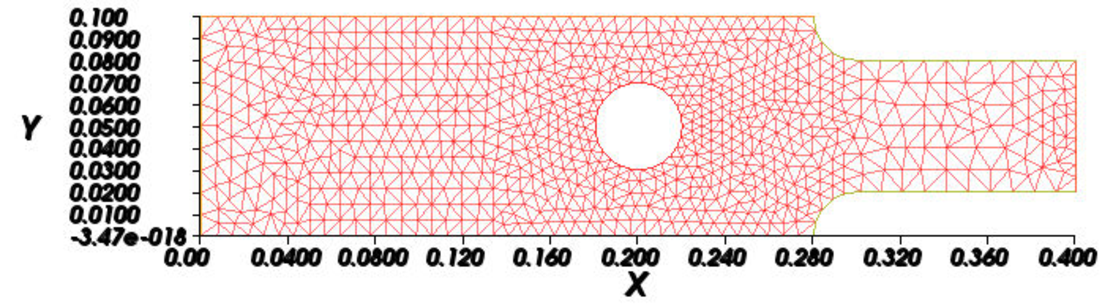
\includegraphics[width=1\textwidth]{paper/4-2-1.pdf}
\caption{Trạng thái ban đầu của tấm kim loại.}
\label{fig:exam21}
\end{figure}\\
Hình dưới đây cho thấy sự biến dạng của tấm kim loại chịu một lực kéo $F = 100$. Do lực kéo là rất nhỏ nên độ biến dạng của tấm kim loại là không lớn \eqref{fig:exam22}.\\
\begin{figure}[http]
\centering
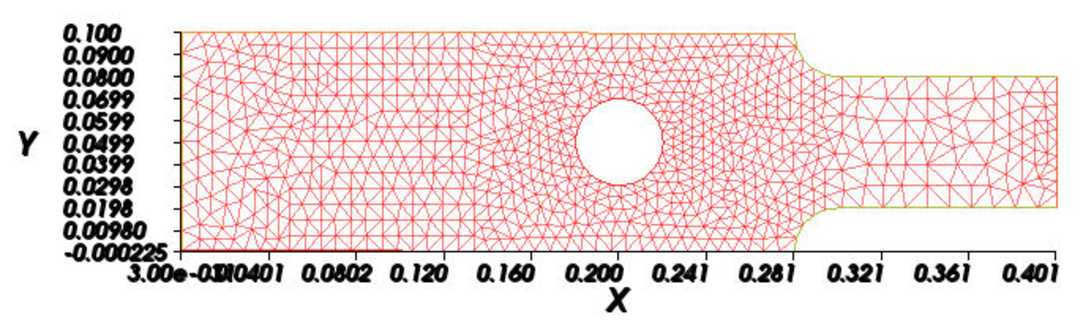
\includegraphics[width=1\textwidth]{paper/4-2-2.pdf}
\caption{Tấm kim loại dưới tác dụng của lực kéo F=100.}
\label{fig:exam22}
\end{figure}\\
Khi ta tăng lực kéo F lên F=5e3 (hình \ref{fig:exam23}) và F=1e4 (hình \ref{fig:exam24}) thì ta thấy độ biến dạng rõ hơn.\\
\begin{figure}[http]
\centering
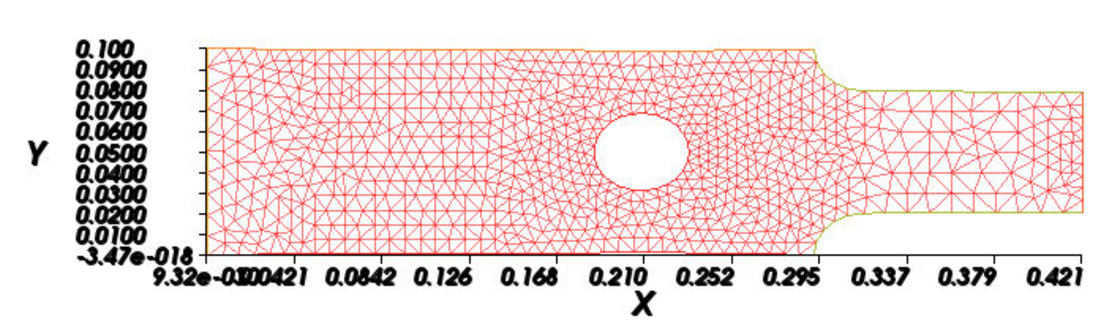
\includegraphics[width=1\textwidth]{paper/4-2-3.pdf}
\caption{Tấm kim loại dưới tác dụng của lực kéo F=5e3.}
\label{fig:exam23}
\end{figure}
\begin{figure}[http]
\centering
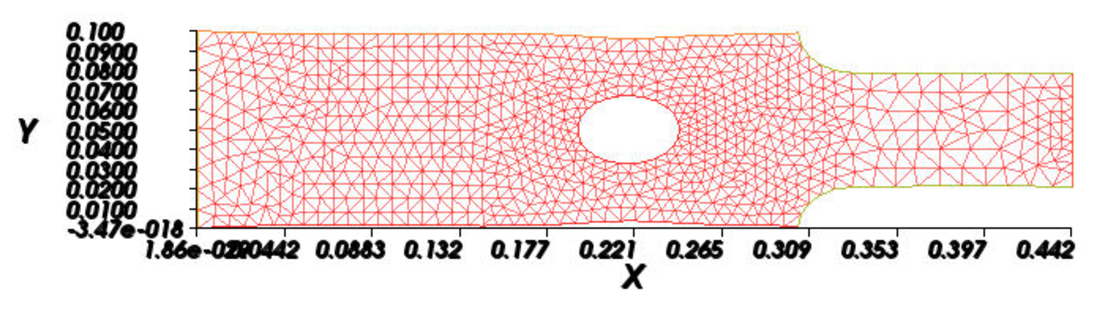
\includegraphics[width=1\textwidth]{paper/4-2-4.pdf}
\caption{Tấm kim loại dưới tác dụng của lực kéo F=1e4.}
\label{fig:exam24}
\end{figure}
\subsection{Mô phỏng thí nghiệm với lực nén}
Xét một tấm kim loại có một lỗ ở giữa chịu tác động của một lực nén $f=(-1e4,0)$ và trọng lực $g=(0,-9.81)$. Cho hằng số mô-đun đàn hồi Young $E=7e4$ và hệ số Poisson $v=0,3$ \cite{TIT-07}. Ta có hình \eqref{fig:exam31} - khởi tạo lưới ban đầu của tấm kim loại và hình \eqref{fig:exam32} - thể hiện lưới biến dạng của tấm kim loại sau khi chịu tác động bởi lực nén.\\
\begin{figure}[http]
\centering
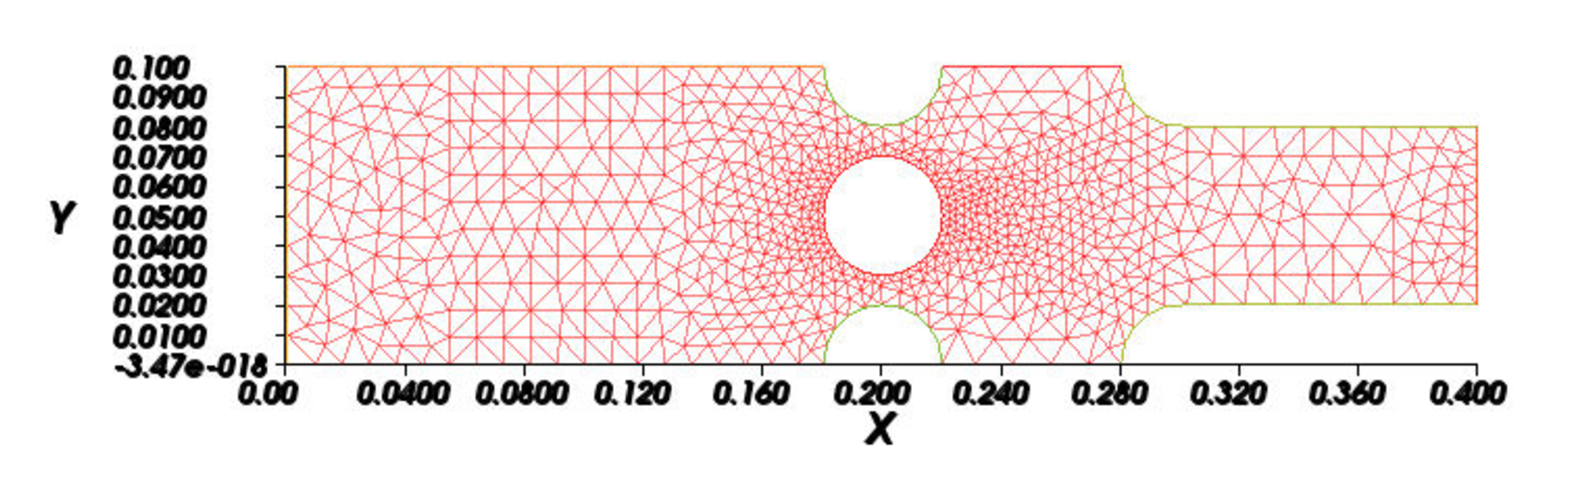
\includegraphics[width=1\textwidth]{paper/4-3-1.pdf}
\caption{Tấm kim loại ở trạng thái ban đầu.}
\label{fig:exam31}
\end{figure}
\begin{figure}[http]
\centering
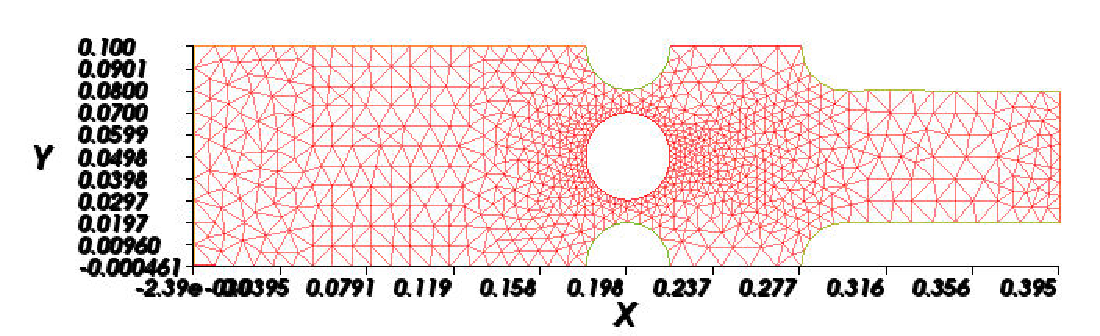
\includegraphics[width=1\textwidth]{paper/4-3-2.pdf}
\caption{Tấm kim loại dưới tác dụng của lực nén.}
\label{fig:exam32}
\end{figure}\\

Xét một tấm kim loại có kích thước là $2 \times 2$ với đáy cố định, chịu tác dụng của một lực nén $f = (0,-1e7)$ lên phía trên của tấm kim loại. Tấm kim loại có một lỗ được cho bởi phương trình $r = 0.5 + 0.2 sin(kt)$ trong tọa độ cực. Trong ví dụ này, ta xét $k=5$. Cho hằng số mô-đun đàn hồi Young và hệ số Poisson lần lượt bằng $E=1e9;\; v=0,3$ \citep{HUI-2011}. Dưới đây là lưới khởi tạo với 5796 tam giác của tấm kim loại \ref{fig:exam33}:\\

\begin{figure}[http]
\centering
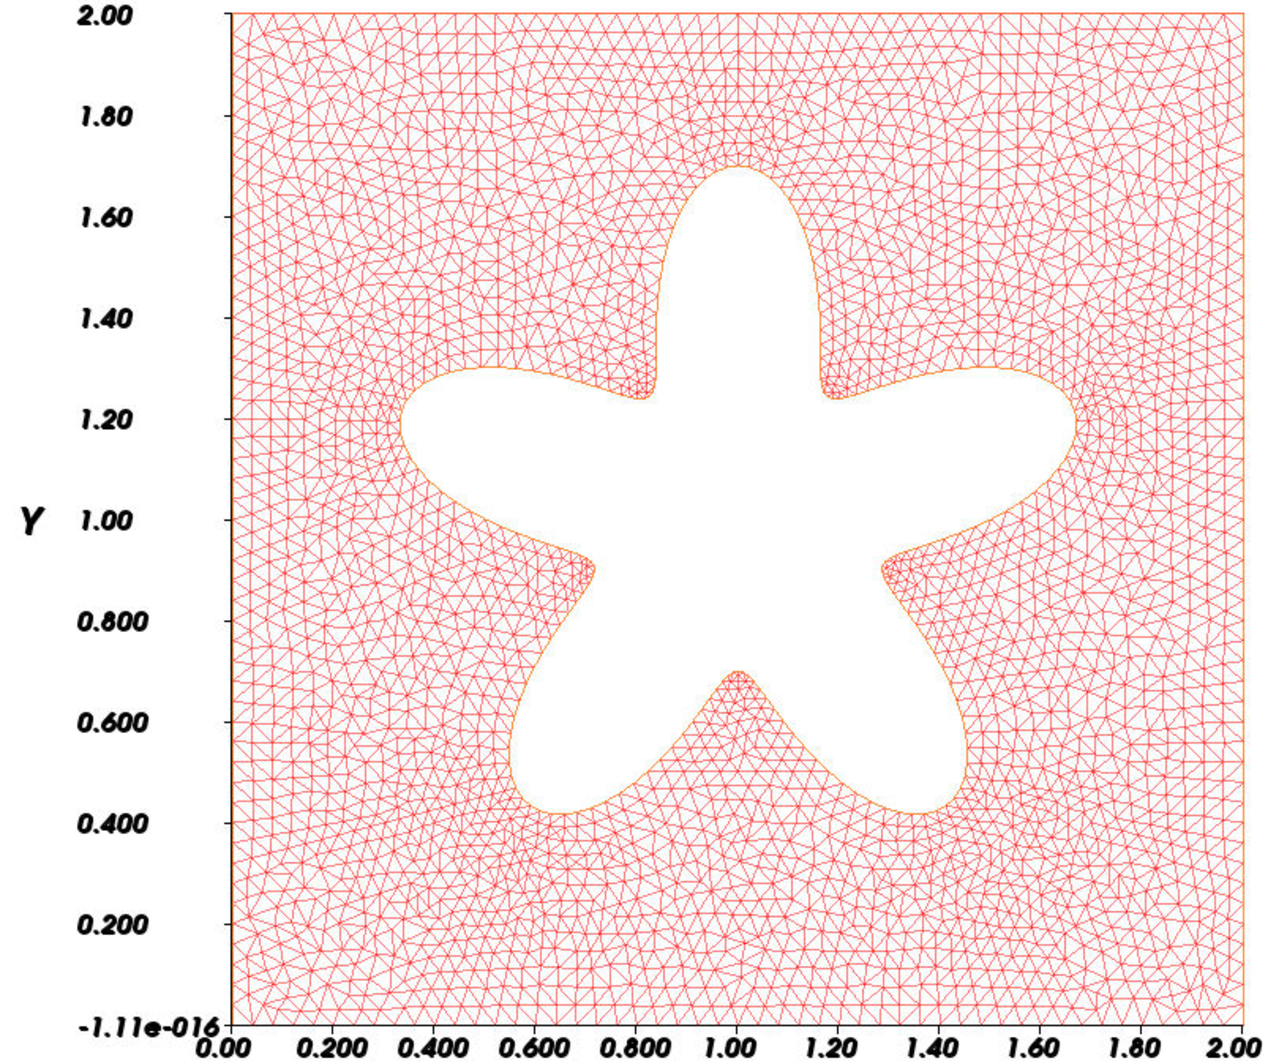
\includegraphics[width=0.6\textwidth]{paper/4-3-3.pdf}
\caption{Tấm kim loại $2 \times 2$ với lỗ $r = 0.5 + 0.2 sin(kt)$.}
\label{fig:exam33}
\end{figure}
Dưới tác dụng của lực nén, tấm sẽ bị nén theo chiều y và phình to ra theo hướng x. Hình sau biểu thị sự dịch chuyển biến dạng của tấm kim loại:\\
\begin{figure}[http]
\centering
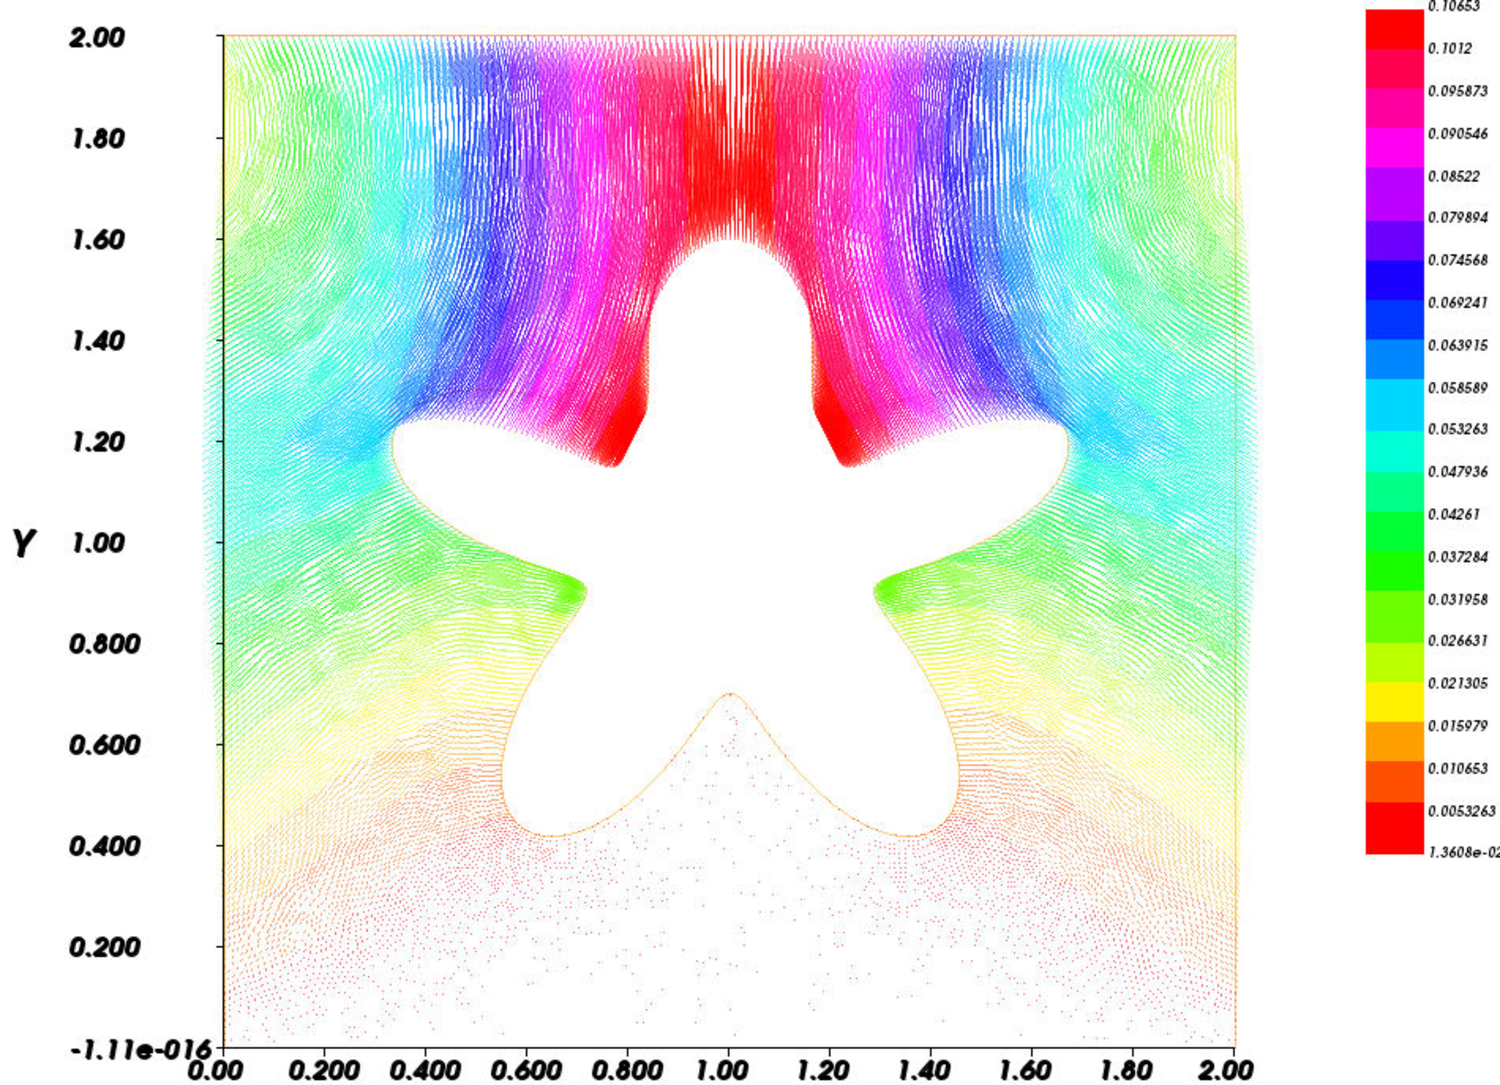
\includegraphics[width=0.6\textwidth]{paper/4-3-4.pdf}
\caption{Hướng dịch chuyển của tấm kim loại.}
\label{fig:exam34}
\end{figure}\\
\begin{figure}[http]
\centering
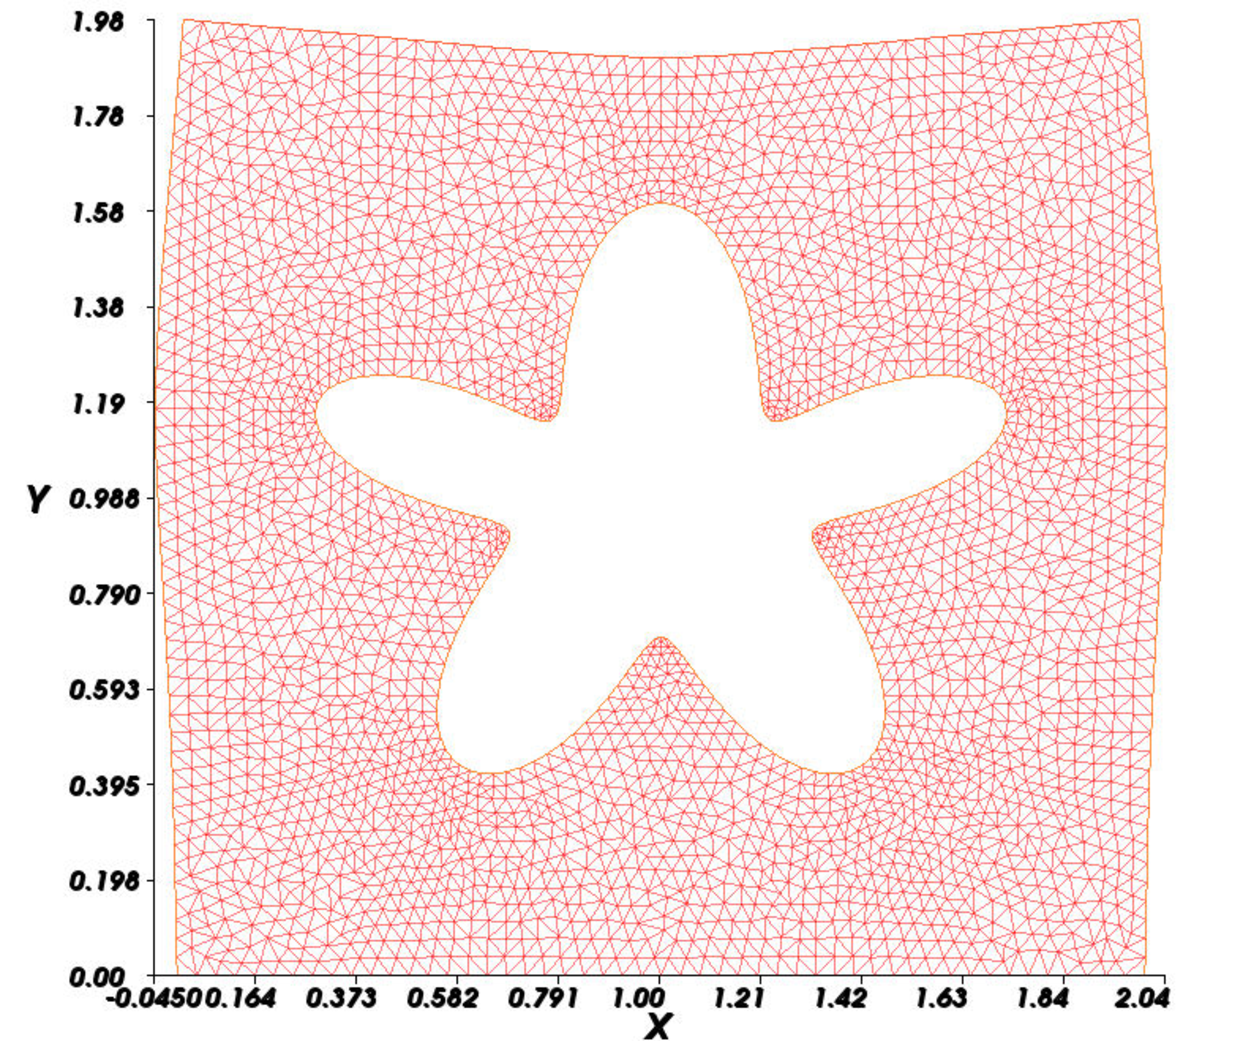
\includegraphics[width=0.6\textwidth]{paper/4-3-5.pdf}
\caption{Tấm kim loại sau khi bị biến dạng.}
\label{fig:exam35}
\end{figure}\\
\subsection{Mô phỏng thí nghiệm với áp suất}
Một tấm kim loại hình khuyên phải chịu một áp lực bên trong như hình \ref{fig:exam41} với $p=1e3;\;E=2e5;\;v=0.3;\;r_i=42;\;r_e=50;\;h=1 (h<<r_i)$ \cite{TIT-07}. Do $(h<<r_i)$ nên ta có thể coi đây là một bài toán 2 chiều. Ở ví dụ tiếp theo, ta xét một ống kim loại có cùng $p, E, v, r_i, r_e$ với chiều dài không nhỏ hơn quá nhiều so với bán kính của ống. Khi đó, bài toán trở thành bài toán 3 chiều.
\begin{figure}[http]
\centering
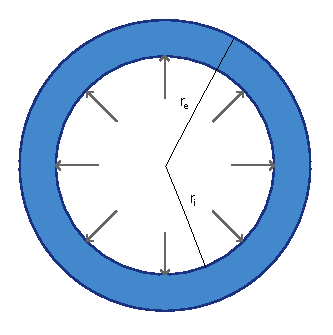
\includegraphics[width=0.6\textwidth]{paper/4-4.pdf}
\caption{Khuyên kim loại chịu tác động của áp suất ở bên trong.}
\label{fig:exam40}
\end{figure}\\
Hình \ref{fig:exam40} biểu diễn trạng thái ban đầu của khuyên kim loại và các lực tác động lên nó. Lưới khởi tạo và sự biến dạng của khuyên kim loại được biểu diễn như trong hình \ref{fig:exam41} \ref{fig:exam42}:
\begin{figure}[http]
\centering
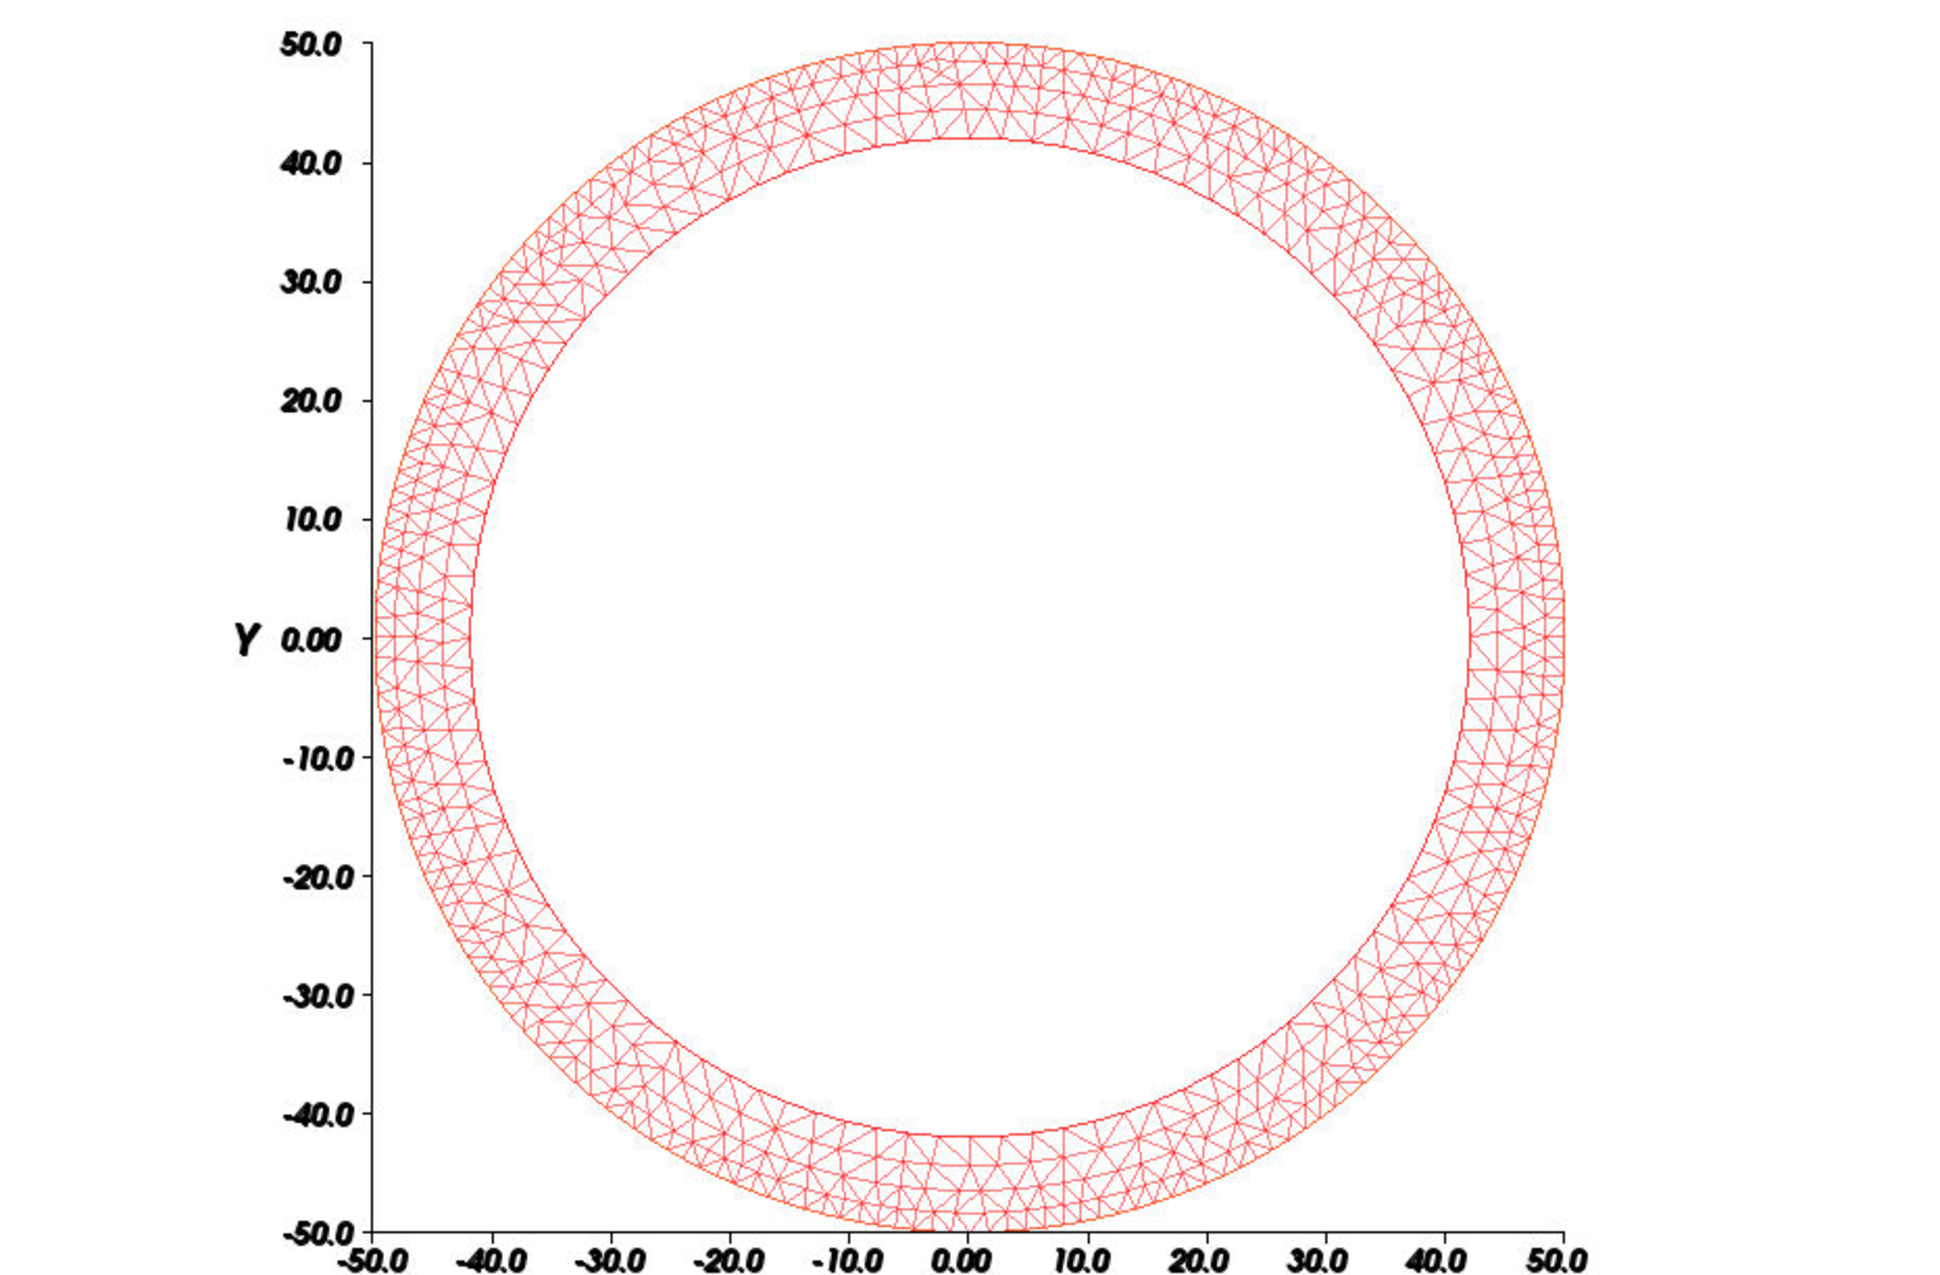
\includegraphics[width=0.6\textwidth]{paper/4-4-1.pdf}
\caption{Lưới khởi tạo của khuyên kim loại.}
\label{fig:exam41}
\end{figure}\\
\begin{figure}[http]
\centering
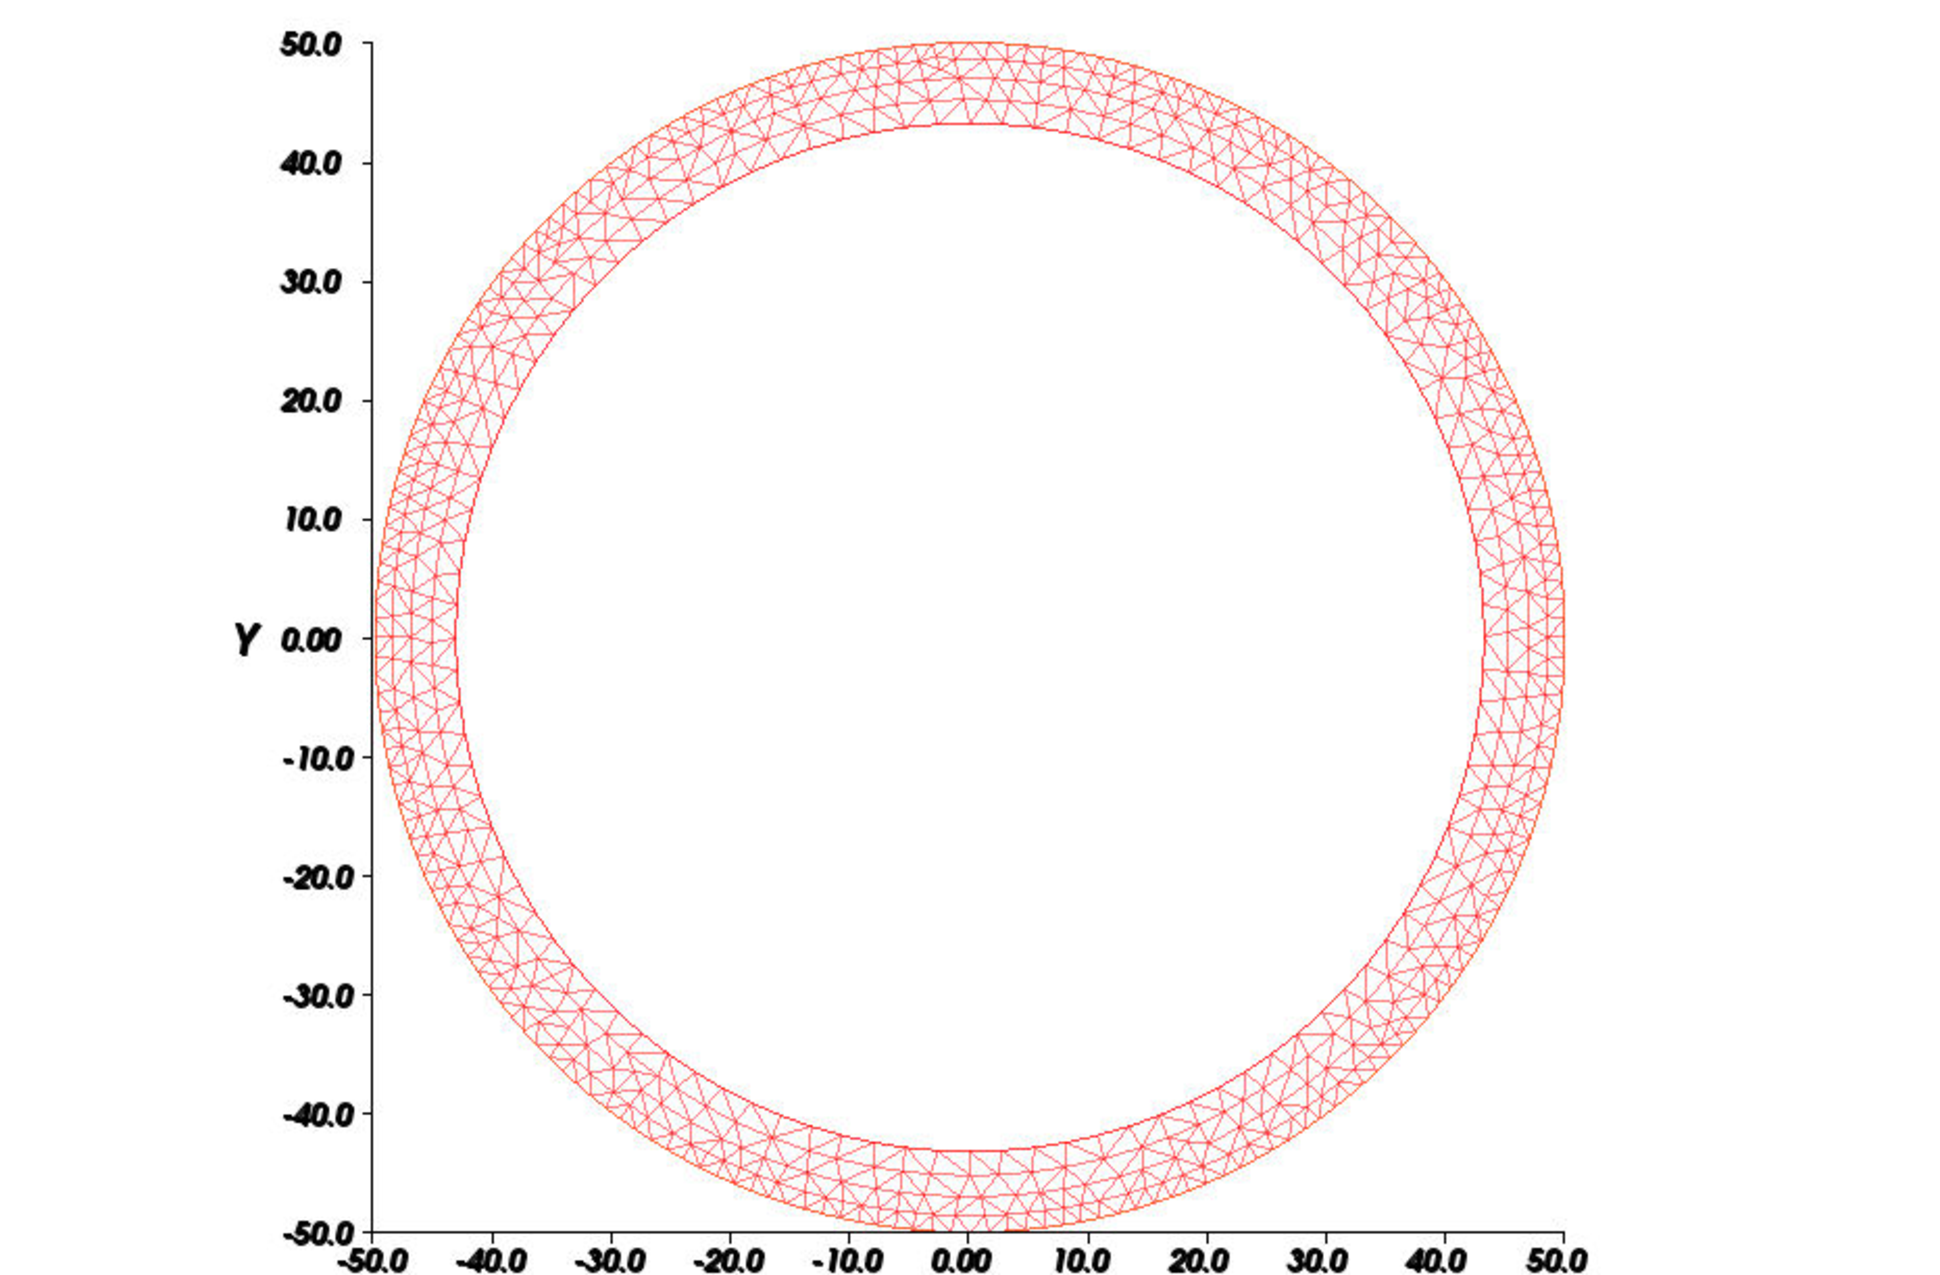
\includegraphics[width=0.6\textwidth]{paper/4-4-2.pdf}
\caption{Sự biến dạng của khuyên kim loại.}
\label{fig:exam42}
\end{figure}\\
Như đã nói ở trên, ta xét một ống kim loại. Có áp suất bên trong ống $p=1e3;\;E=2e5;\;v=0.3;\;r_i=40;\;r_e=50$ và ống có chiều dài $h=40$.\\
\begin{figure}[http]
\centering
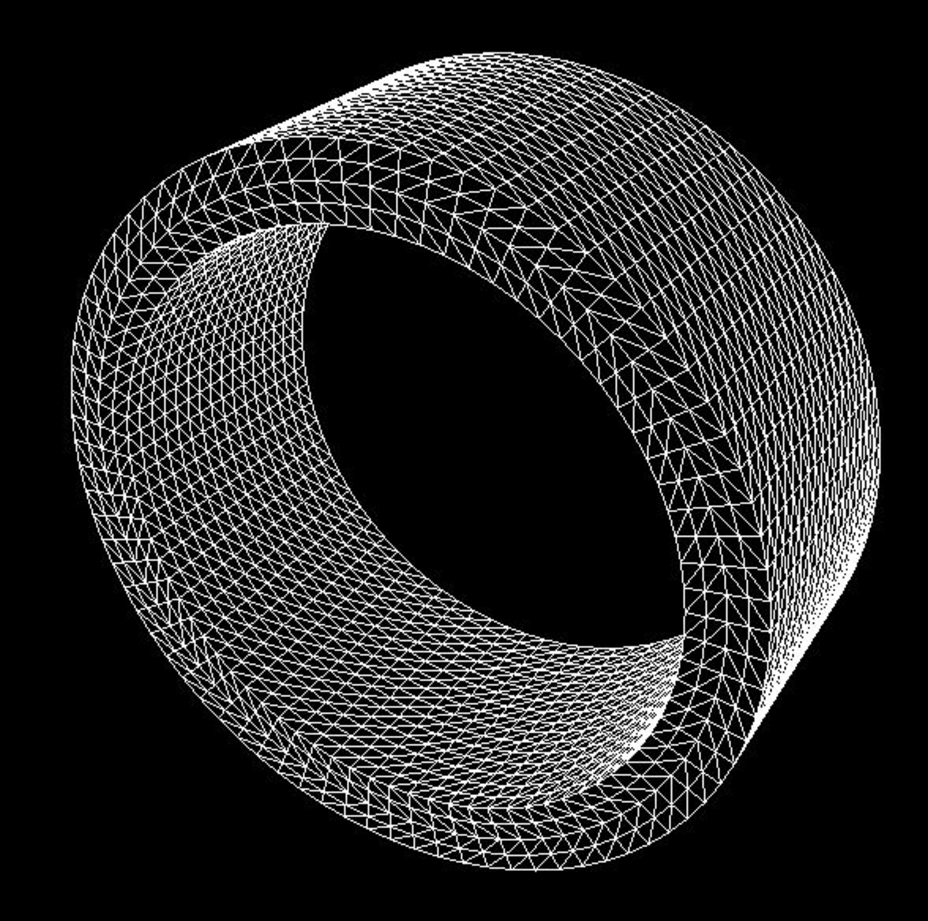
\includegraphics[width=0.6\textwidth]{paper/4-5.pdf}
\caption{Lưới khởi tạo của ống kim loại.}
\label{fig:exam50}
\end{figure}\\
Và các hình \ref{fig:exam51}, \ref{fig:exam52} cho thấy sự biến dạng của ống kim loại:
\begin{figure}[http]
\centering
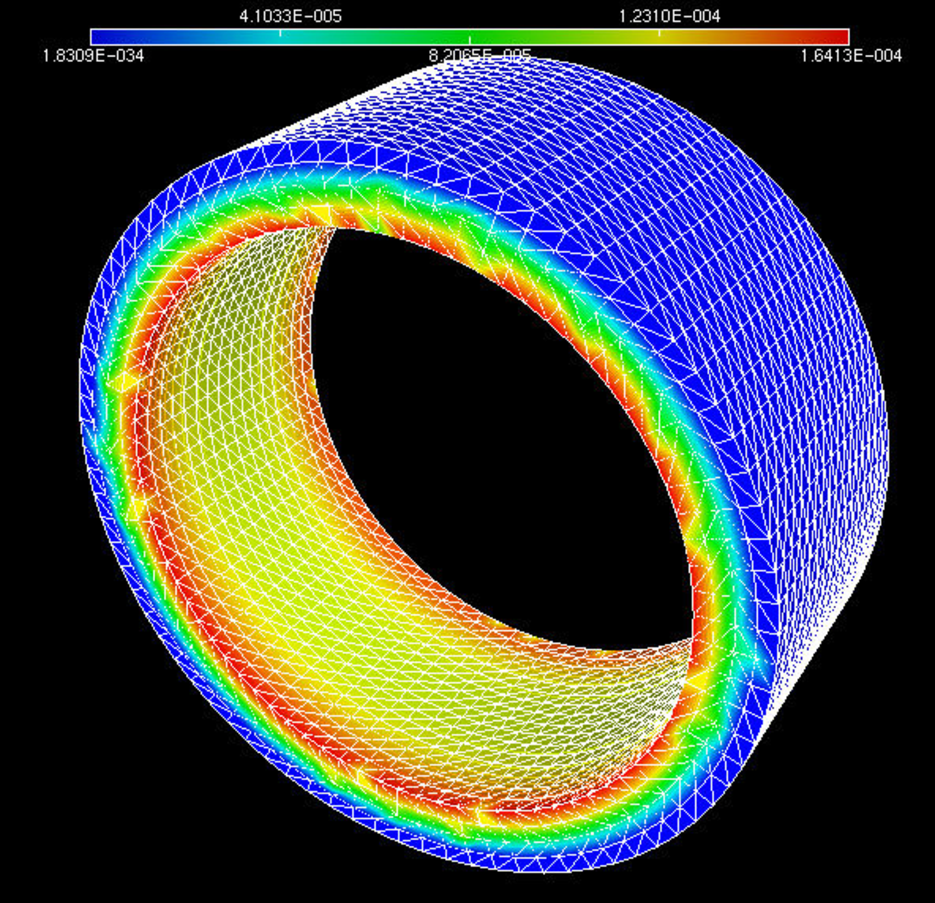
\includegraphics[width=0.6\textwidth]{paper/4-5-1.pdf}
\caption{Ống kim loại trước khi bị biến dạng.}
\label{fig:exam51}
\end{figure}\\
\begin{figure}[http]
\centering
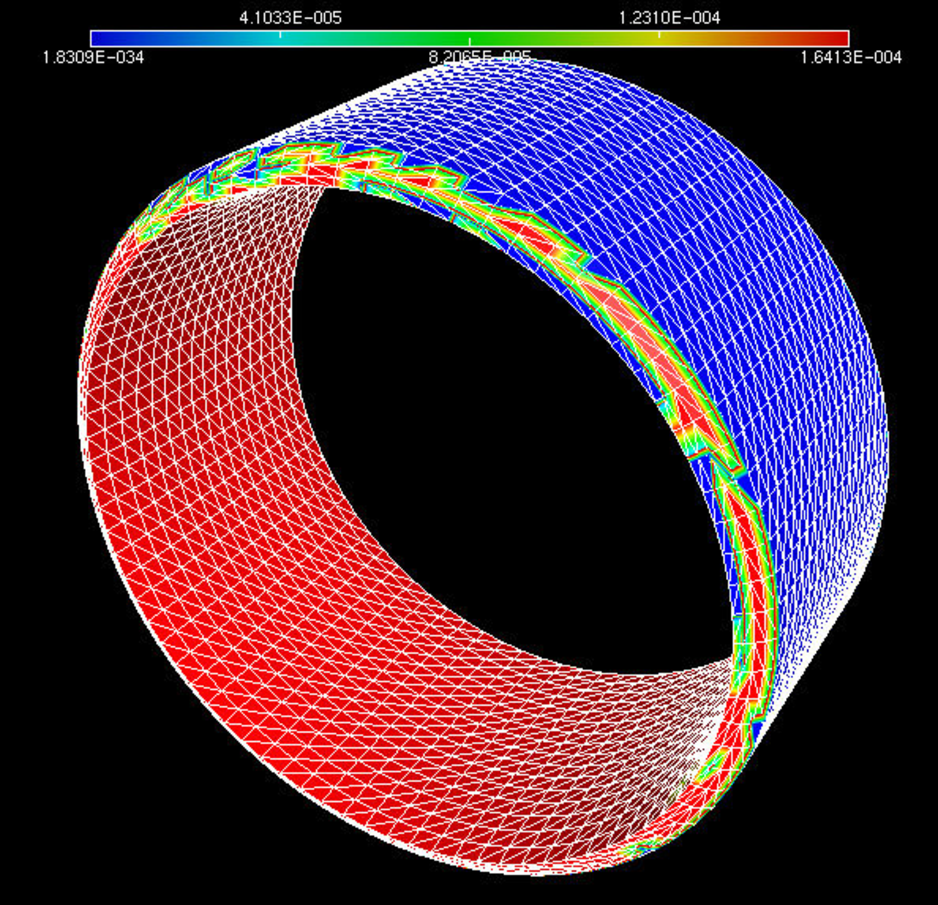
\includegraphics[width=0.6\textwidth]{paper/4-5-2.pdf}
\caption{Ống kim loại sau khi bị biến dạng.}
\label{fig:exam52}
\end{figure}\\

\section{Kết luận}
Trong chương này, ta đã trình bày chi tiết các bước xây dựng lược đồ giải số cho hệ phương trình biến dạng đàn hồi. Cụ thể, nội dung chương \ref{Chapter1} đã giải quyết những vấn đề sau:
\begin{itemize}
\item Phát biểu bài toán biến dạng đàn hồi.
\item Áp dụng phương pháp phần tử hữu hạn rời rạc hóa không gian, từ đó xây dựng bài toán rời rạc và hệ phương trình đại số tương ứng.
\item Trình bày các ví dụ giải số minh họa.
\end{itemize}

%----------------------------------------------------------------------------------------
% Chapter 2
\chapter{Ứng dụng trong công nghiệp vật liệu}\label{Chapter2}
\renewcommand{\baselinestretch}{1.25}
\minitoc
\renewcommand{\baselinestretch}{1.5}
%----------------------------------------------------------------------------------------
\section{Ứng dụng trong bài toán tối ưu dạng}
Trong sản xuất vật liệu công nghiệp, việc chọn được thành phần và thiết kế cấu trúc là một phẩn rất quan trọng để sản xuất các sản phẩm bền vững và mang tính cạnh tranh. Để đáp ứng các yêu cầu về độ bền của vật liệu, việc tối ưu hóa cấu trúc và cấu tạo của vật liệu được sử dụng quá trình thiết kế. Trong việc thiết kế vật liệu dựa trên tối ưu hóa hình dạng, thách thức chính ở đây là tuân theo hình dạng được đề xuất mà không tạo ra các biến thể phần thì quá mỏng dẹt hay phần thì quá dày quá dày gây nên mất hình dạng cấu trúc của vật. Do đó, tối ưu hình dạng vật liệu góp phần không nhỏ trong việc sản xuất vật liệu. Trong chương này của luận văn, phần đầu sẽ sẽ giới thiệu về bài toán tối ưu hình dạng của vật có cấu trúc đàn hồi và sau đó là một vài ví dụ mô phỏng số trong việc thiết kế cấu tạo của một số vật liệu.
\subsection{Bài toán tối ưu dạng}
Bài toán tối ưu dạng là bài toán tìm hình dạng tối ưu $\Omega^*$ của vật thể trong tập các hình dạng chấp nhận được $\Omega_x\subset\mathbb{R}^n$ theo một tiêu chí xác định nào đó và được mô tả thông qua việc cực tiểu hàm mục tiêu $J:\Omega_x\rightarrow\mathbb{R}$. Xét bài toán tối ưu dạng:
\begin{equation}\label{bt:toiuidang}
\inf_{\Omega\in\Omega_x}J(\Omega)
\end{equation}
Trong từng bài toán tối ưu dạng cụ thể, ta có được hàm mục tiêu $J(\Omega)$ khác nhau tương ứng trong các trường hợp đó. Chẳng hạn, khi ta cần tối ưu dạng của một đường ống (hình \ref{fig:exampipe}), ta quan tâm đến tổng công của dòng chảy được sinh ra bên trong ống:
$$J(\Omega) = 2\mu\int_\Omega D(u_\Omega):D(u_\Omega)dx.$$
\begin{figure}[http]
\centering
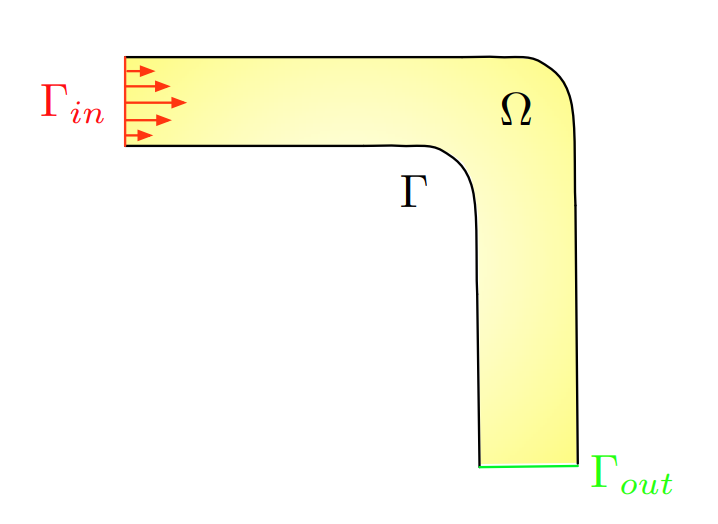
\includegraphics[width=0.6\textwidth]{exampipe.png}
\caption{Hình dạng ban đầu của đường ống.}
\label{fig:exampipe}
\end{figure}\\
Trong bài toán này, ta có thêm ràng buộc về thể tích cần đạt được cho đường ống để khống chế hình dạng tối ưu của đường ống.\\
Hàm bình phương sai số cũng là một hàm mục tiêu được xét nhiều trong các bài toán tối ưu hình dạng của các vật liệu. Ví dụ như ta xét một dòng chảy trên miền D, trong dòng chảy đó có một vật cản $\omega$ có hình dạng không xác định. Gọi $u_{meas}$ là vận tốc của dòng chảy $u_\Omega$ ở vị trí $\mathcal{O}$ với mục đích  tái cấu trúc hình dạng của vật cản $\omega$(hình \ref{fig:examdcvc}). Khi đó miền tối ưu là $\Omega = D\backslash\omega$ và chỉ phần $\partial\omega$ của $\partial\Omega$ là được tối ưu. Mục tiêu là ta cần tối thiểu hàm bình phương sai số:
$$J(\Omega)=\int_\mathcal{O}|u_\Omega - u_{meas}|^2dx.$$
\begin{figure}[http]
\centering
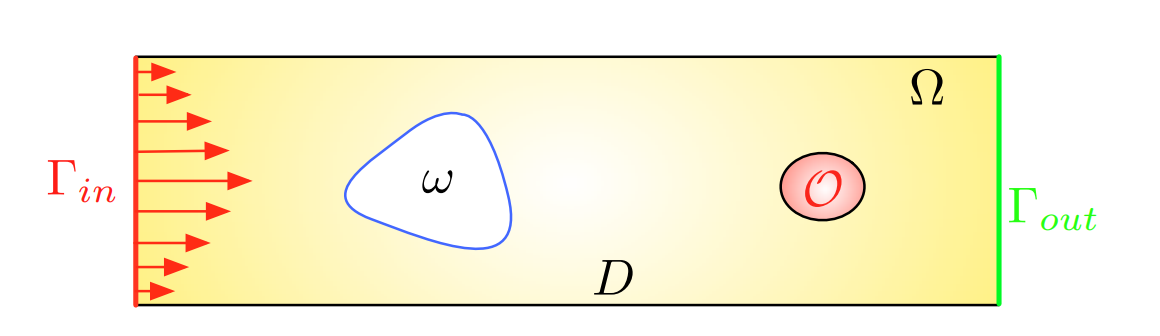
\includegraphics[width=0.8\textwidth]{examdcvc.png}
\caption{Dòng chảy trên miền $D$ có vật cản $\omega$ ở giữa.}
\label{fig:examdcvc}
\end{figure}\\
Trong ngành công nghiệp hàng không, hàm mục tiêu ở đây là ta cần tối ưu lực kéo $\mathcal{T}$ của cánh $\Omega$ \cite{Pir84, MP10}:
$$J(\Omega)=\mathcal{T}(\Omega)=\int_\Om \left[\mu \left(\nabla u + \nabla u^T\right) - \frac{2\mu}{3} \Div u \right]\nv \,dx  - \int_\Om p\nv \,dx.$$
Trong luận văn này, ta sẽ tìm hiểu rõ hơn về hàm mục tiêu dạng mô tả tính đàn hồi được áp dụng trong các bài toán tối ưu hóa hình dạng, cấu trúc vật liệu:
\begin{equation}\label{eq:hmt}
J(\Omega)=\int_\Omega f\cdot u\,dx + \int_{\Gm_N} g \cdot u \,ds = \int_{\Om} Ae(u):e(u)\,dx.
\end{equation}

\subsection*{Các điều kiện ràng buộc}
Trong các ví dụ ở trên, ta có đề cập đến ràng buộc về thể tích tối ưu cần đạt được giúp ta khống chế được hình dạng cũng như cấu trúc của vật liệu. Ngoài ràng buộc về thể tích ra, trong bài toán tối ưu hình dạng của vật liệu, ta còn có điều kiện về chu vi dạng hay tổng độ cong biên.
\begin{itemize}
\item Thể tích dạng: $\text{Vol}(\Omega)=\int_\Omega dx$
\item Chu vi dạng: $\text{Per}(\Omega)=\int_{\partial\Omega} ds$
\item Tổng độ cong biên: $\mathcal{K}(\Omega)=\int_\Omega\kappa^2ds$
\end{itemize}
Đó là các hàm dạng phổ biến được sử dụng, đóng vai trò quan	 trọng việc hiệu chỉnh các thành phần của vật liệu cũng như tái cấu trúc hình dạng vật liệu.\\
Để xử lý các điều kiện ràng buộc như đã đề cập ở trên, ta đưa nhân tử Lagrange $l$ vào hàm mục tiêu phương pháp đó còn gọi là phương pháp Lagrange tăng cường (Augmented Lagrange method) dùng để giải các bài toán tối ưu có ràng buộc, được trình bày trong nghiên cứu của Magnus R. Hestenes năm 1969 \cite{Hes69}. 
\subsection*{Phương pháp biến phân Hadamard}
Phương pháp biến phân Hadamard được đề xuất trong các nghiên cứu \cite{Had07, SZ92}. Sau đó ý tưởng của phương pháp này được Murat và Simon phát triển tiếp \cite{MS76a, Sim80}. Dựa trên cách tiếp cận phương pháp biến phân Hadamard có trong \cite{MS76a, Sim80}, cho trước một trường dịch chuyển $\tta \in W^{1,\infty}(\mathbb{R}^d,\mathbb{R}^d)$ đủ nhỏ, ta xét biến phân của một dạng trơn $\Om$ theo trường dịch chuyển đó, được cho bởi công thức $\Om_\tta = (I+\tta)(\Om)$ (hình \ref{fig:shapeVariation}). Do đó, biến phân $(I+\tta)$ là một phép vi phôi "gần" với ánh xạ đồng nhất.
\begin{figure}[http]
\centering
\centering
\begin{tikzpicture}[scale = 0.9]
\coordinate [label={[black] \small $x$}] (A) at (0.7,0.2);
\coordinate (B) at (0,1.5);
\coordinate (C) at (0.5,3);
\coordinate (D) at (2,4);
\coordinate (E) at (5,5);
\coordinate (F) at (5.7,4);
\coordinate (G) at (7,1.9);
\coordinate (H) at (4.5,0.3);
\coordinate (I) at (3,0.5);
\coordinate (J) at (2,0.6);
\coordinate (K) at (1.5,0.5);

\coordinate [label = {[red] below:\small $\tta(x)$}] (A') at (0.7,-0.2);
\coordinate (B') at (-0.3,1.5);
\coordinate (C') at (0.5,3.5);
\coordinate (D') at (2.6,4);
\coordinate (E') at (3.5, 4.8);
\coordinate (F') at (5,5.2);
\coordinate (G') at (7.2,2.1);
\coordinate (H') at (5.5,1);
\coordinate (I') at (4.5,0.1);
\coordinate (J') at (3,0.3);
\coordinate (K') at (2,0.4);

\draw [line width=0.3mm, black] plot [smooth cycle] coordinates {(A) (B) (C) (D) (E) (F) (G) (H) (I) (J) (K)};
\draw [line width=0.5mm, red, dotted] plot [smooth cycle] coordinates {(A') (B') (C') (D') (E') (F') (G') (H') (I') (J') (K')};

\begin{scope}[on background layer]
\fill[white!20!, opacity=.5] plot [smooth cycle] coordinates {(A') (B') (C') (D') (E') (F') (G') (H') (I') (J') (K')};
\fill[white!30!, opacity=.5] plot [smooth cycle] coordinates {(A) (B) (C) (D) (E) (F) (G) (H) (I) (J) (K)};
\end{scope};

\draw[line width=0.4mm, -latex, red, label={[red] below: $\tta(x)$}] (A) -- (A');

\node at (4.5,0.6) {\small $\Om$};
\node at (0.5,4.5) [label={[red] below: \small $(I+\tta)(\Om)$}] {};
\end{tikzpicture}
\caption{Biến phân $(I + \tta)$ của một dạng $\Om$ cho trước.}
\label{fig:shapeVariation}
\end{figure}\\
Trong phương pháp Hadamard, biến phân $(I+\tta)$ của dạng $\Om$ chỉ phụ thuộc vào giá trị của $\tta$ xác định trên biên $\pa\Om$. Do đó, từ định lý điểm bất động Picard (xem chứng minh trong \cite{All06}) ta có hệ quả sau:
\begin{lem}[Bổ đề 6.13 trong \cite{All06}] Với mỗi trường biến dạng $\tta \in W^{1,\infty}(\R^d,\R^d)$ thỏa mãn $\:\norm{\tta}_{W^{1,\infty} (\mathbb{R}^d,\mathbb{R}^d)}<1$, ánh xạ $(I+\tta):\R^d\ra\R^d$ là một phép đồng phôi Lipschitz với nghịch đảo Lispchitz.
\end{lem}
Với mọi $\theta \in W^{1,\infty}(\R^d,\R^d),\: \norm{\tta}_{W^{1,\infty} (\mathbb{R}^d,\mathbb{R}^d)}<1$ ta định nghĩa $\Omega_\theta = (I+\tta)(\Omega)$ là biến phân của $\Omega$ dịch chuyển theo $\theta$. Chú ý rằng $W^{1,\infty}(\R^d,\R^d) \subset L^\infty(\R^d)^d$ là không gian Banach các hàm $\tta : \R^d \ra \R^d$ với chuẩn:
$$\forall\theta \in W^{1,\infty}(\R^d,\R^d), \: \norm{\tta}_{W^{1,\infty} (\mathbb{R}^d,\mathbb{R}^d)} := \norm{\tta}_{L^\infty(\R^d)^d} + \norm{\na\tta}_{L^\infty(\R^d )^{d\times d}}.$$
Do đó, các biến phân của dạng $\Omega$ cho trước được biểu diễn bằng một tập con mở của không gian Banach. Ở trong phần tiếp theo, phương pháp biến phân Hadamard sẽ định nghĩa lại khái niệm khả vi dạng thông qua phép biến dạng $(I+\tta)$.
\subsection*{Tính khả vi dạng}
Theo cách tiếp cận của Murat và Simon \cite{MS76a, Sim80}, bắt đầu từ một dạng trơn $\Omega$, như ở phần trước ta có biến phân $\Om_\tta = (I+\tta)(\Om)$ với $\tta \in W^{1,\infty}(\mathbb{R}^d,\mathbb{R}^d)$. Nên trong phần này ta sẽ nói về đạo hàm của một số hàm dạng $\Om \mapsto J(\Om)\in\R$.
\begin{defi}\label{def:dhd}
Cho $J(\Om)$ là một hàm dạng. $J$ được gọi là khả vi dạng tại $\Om$ nếu ánh xạ:
\begin{align*}
W^{1,\infty}(\R^d,\R^d) &\lra \R\\
\tta &\map J(\Om_{\tta})
\end{align*}
là khả vi Fr\'echet tại $\tta=0$. Đạo hàm Fr\'echet tương ứng, ký hiệu là $J'(\Om)(\tta)$, được gọi là đạo hàm dạng của $J$ tại $\Om$. Ta có khai triển của $J(\Om_\tta)$ tại lân cận $0 \in W^{1,\infty}(\R^d,\R^d)$:
\begin{equation}\label{eq:dhd}
J(\Om_{\tta})=J(\Om)+J'(\Om)(\tta)+o(\tta), \quad \text{trong đó  } \, \lim_{\tta\ra 0}\,\dfrac{|o(\tta)|}{\norm{\tta}_{W^{1,\infty}(\R^d,\R^d)}} = 0.
\end{equation}
\end{defi}

\begin{rem}\leavevmode
\begin{enumerate}[noitemsep,topsep=0pt]
	\item $J'(\Om)$ là dạng tuyến tính liên tục trên $W^{1,\infty}(\R^d,\R^d)$.
	\item Trong trường hợp hàm nhiều biến, đạo hàm riêng Fr\'echet theo biến dạng được ký hiệu là $\frac{\pa}{\pa{\Om}}$.
\end{enumerate}
\end{rem}

Hai kết quả trên của đạo hàm dạng sẽ được sử dụng trong các tính toán ở phần sau (chứng minh chi tiết của hai kết quả trên có thể xem tại \cite{AJT04} hoặc \cite{HP18}).

\begin{lem}[Định lý 5.2.2 trong \cite{HP18}] \label{lem:31}
Cho $\Om$ là một miền bị chặn Lispchitz trong $\R^d$ và $f(x) \in W^{1,1}(\R^d)$. Nếu $J(\Om)=\int_{\Om}f(x)\,dx$ thì $J$ là hàm khả vi dạng tại $\Om$ và với mỗi $\tta \in W^{1,\infty}(\R^d,\R^d)$:
$$J'(\Om)(\tta)=\int_{\Om} \Div (\tta f)\,dx=\int_{\pa{\Om}} f \tta\cdot\nv \,ds. $$
\end{lem}

\begin{lem}[Định lý 5.4.17 trong \cite{HP18}]\label{lem:32}
Cho $\Om$ là một miền bị chặn Lipschitz trong lớp $\CC^2$ và $g(x) \in W^{2,1}(\R^d)$. Nếu $J(\Om)=\int_{\pa{\Om}}g(x)\,ds$ thì $J$ là hàm khả vi dạng tại $\Om$ và với mỗi $\tta \in W^{1,\infty}(\R^d,\R^d)$:
$$ J'(\Om)(\tta)=\int_{\pa{\Om}} \left( \frac{\pa{g}}{\pa{\nv}}+\kappa g \right) \tta\cdot\nv \,ds, $$
trong đó $\kappa$ là độ cong trung bình của biên $\pa{\Om}$, được định nghĩa bởi $\kappa= \Div \nv$.
Hơn nữa, kết quả này vẫn đúng nếu thay $\pa{\Om}$ bởi $\Gm$ là một tập con mở, trơn của $\pa{\Om}$, với giả sử rằng $g = 0$ trên ranh giới bề mặt của $\Gm$.
\end{lem}
Chứng minh chi tiết hai bổ đề trên xem trong \cite{HP18}.
\begin{rem}
Một hệ quả trực tiếp từ bổ đề \eqref{lem:31}, ta có thể tính đạo hàm dạng của hàm thể tích:
\begin{equation}\label{eq:volD}
\Vol(\Om)=\int_\Om \,dx \: \text{và} \: \Vol'(\Om)(\tta)=\int_{\pa\Om}\tta(x)\cdot\nv(x)\,ds.
\end{equation}

Tương tự, bổ đề \eqref{lem:32} cho phép tính đạo hàm dạng của hàm chu vi:
\begin{equation} \label{eq:perD}
\Per(\Om)=\int_{\pa \Om} \,ds \: \text{và} \: \Per'(\Om)(\tta)=\int_{\pa\Om}\kappa \tta(x)\cdot\nv(x)\,ds.
\end{equation}
\end{rem}

\subsection*{Đạo hàm dạng của hàm mục tiêu}
Giả sử $\Omega$ là miền của một vật dẳng hướng tuyến tính. Chúng ta giả sử rằng $\Omega$ cố định trên biên $\Gamma_D$, tác dụng một lực $g$ lên trên biên $\Gamma_N$ và phần biên cần phải tối ưu là $\Gamma_{opt}$, với $\partial\Omega = \Gamma_D\cup\Gamma_N\cup\Gamma_{opt}$. Sự biến dạng của vật thể là nghiệm của phương trình đàn hồi:
\begin{equation}\label{probdhd}
\quad\quad\quad\quad\quad
\begin{cases}
\text{div}(\mathcal{A}(u)) = 0 \qquad \text{trong } \Omega,\\
u = 0 \quad\qquad\qquad\qquad \text{trên } \Gamma_D, \\
\mathcal{A}(u)n = g \qquad\qquad \text{trên } \Gamma_N \\
\mathcal{A}(u)n = 0 \qquad\qquad \text{trên } \Gamma_{opt}.
\end{cases}
\end{equation}
Chúng ta cần tối ưu hóa hình dạng của vật thể trên với thể tích cố định cho trước.  Kết hợp với \ref{eq:hmt} và \ref{probdhd} ta có bài toán tối ưu ràng buộc:
$$\min_\Omega J(\Omega) = \int_{\Gamma_N}g.u(\Omega)ds$$
trên tát cả các tập mở $\Omega$ thỏa mãn $\Gamma_N\cup\Gamma_D\subset\partial\Omega$ có thể tích là $V_0$.\\
Ta có đạo hàm dạng của hàm mục tiêu $J(\Omega)$:
$$<J'(\Omega), \theta> = -\int_{\Gamma_{opt}}(2\mu|e(u(\Omega))|^2+\lambda(\text{div}\;u(\Omega))^2)(\theta.n)ds.$$
\subsection{Thuật toán tối ưu dạng}
\subsubsection*{Phương pháp gradient giải bài toán tối ưu}
Phương pháp gradient là một thuật toán giải bài toán tối ưu dựa trên đạo hàm bậc nhất để xác định hướng giảm của hàm mục tiêu.\\
Cho $F$ là một ánh xạ từ một không gian Hilbert $X$ vào $\mathcal{R}$. Phương pháp gradient được sử dụng để xây dựng một chuỗi các phần tử $(x_n)_{n\geq 0}\in X$:
$$x_{n+1} = x_n - h_nd_n$$
với $h_n \in\mathcal{R}$ là một số dương nhỏ và $d_n$ được định nghĩa như sau:
$$(d_n , y )_X  = \langle F'(x_n),y \rangle_{X * , X} \; \forall y \in X$$
Trong trường hợp này $d_n$ chính là gradient của $F$, hay $d_n = F'_{x_n}$. Nếu $F'(x_n) \neq 0$ và $h_n$ đủ nhỏ thì $F(x_n + 1) < F(x_n)$. Nếu $F$ là hàm lồi mạnh thì tồn tại $x_*$ thỏa mãn:
$$F(x_*)=\min_{x\in X}F(x)$$
Trong tối ưu dạng, tập $X$ không phải là một không gian Hilbert mà là một tập con của $\mathcal{R}^N$ (với $N=2$ hoặc $N=3$) và cũng không dễ dàng để có thể tính đạo hàm. Tuy nhiên, phương pháp gradient vẫn có thể áp dụng một cách hiệu quả.
\subsubsection*{Tính toán hướng giảm gradient}
\begin{itemize}
\item Chọn điểm bắt đầu $x_0$
\item Lặp cho đến khi nghiệm hội tụ hoặc $n=n_{\text{max}}$
\begin{itemize}
\item Xác định $d_n = \nabla F$
\item Tính $x_{n+1} = x_n - h_n d_n$ với $h_n > 0$ bé.
\end{itemize}
\end{itemize}
\subsubsection*{Tối ưu hàm mục tiêu}
Để có thẻ áp dụng phương pháp gradient cho tối ưu dạng, ta cần phải tìm được hướng giảm $d$ dựa vào đạo hàm dạng $J'(\Omega)$. Trong trường hợp này, xét không gian $H^1(\Omega)^N$, hướng giảm $d \in H^1(\Omega)^N$ thỏa mãn với mọi $\theta \in H^1(\Omega)^N$, ta có:
\begin{equation}\label{btdhd}
\int_\Omega (\nabla d.\nabla \theta + d.\theta)dx=<J'(\Omega),\theta>
\end{equation}
Ta thực hiên tối ưu hàm mục tiêu bằng phương pháp gradient theo các bước sau:
\begin{itemize}
\item Chọn dạng khởi đầu $\Omega_0$
\item Lặp cho đến khi hội tụ với $n\geq 0$
\begin{itemize}
\item Tính toán $d_n$ là kết quả của bài toán \ref{btdhd} với $\Omega = \Omega_n$.
\item Đặt $\Omega_{n+1} = (I-h_n d_n)(\Omega_n)$ với $h_n$ là một bước nhỏ.
\end{itemize}
\end{itemize}
\subsubsection*{Phương pháp Lagrange giải quyết ràng buộc thể tích}
Nhiều bài toán tối ưu dạng đặt ra ràng buộc về thể tích của vật. Để xử lý ràng buộc này, như đã đề cập ở phần trước, ta sẽ đưa nhân tử Lagrange $l$ vào hàm mục tiêu. Cụ thể hơn, ta có thể tính hướng giảm bằng hướng giảm của phương trình Lagrange $J'(\Omega) + lV'(\Omega)$, với $V(\Omega) = |\Omega|$ là thể tích của dạng $\Omega$. Giá trị của nhân tử Lagrange được đặt lại tại mỗi vòng lặp, do đó, hình dạng sẽ luôn thỏa mãn điều kiện ràng buộc về mặt thể tích. Tại mỗi thời điểm, nếu giá trị thể tích hiện tại lớn hơn giá trị thể tích dự kiến, ta sẽ tăng giá trị của nhân tử Lagrange và tương ứng ngược lại, giảm nếu giá trị thể tích hiện tại nhỏ hơn giá trị dự kiến. Tuy nhiên, cách này dẫn đến sự dao động của thể tích dạng. Do đó, ta nới lỏng nó với giá trị của nhân tử Lagrange được tính toán với giả thiết điều kiện tối ưu đã thỏa mãn, tức là $J'(\Omega) + lV'(\Omega) = 0$. Chi tiết hơn ta có:
$$l^{n+1}=(l^n+l)/2 + \epsilon_l(V-V_0)$$
với $\epsilon_l$ đủ nhỏ.
\subsubsection{Xác định bước giảm $h_n$}
Việc chon $h_n$ là một yếu tố ảnh hưởng trực tiếp đến tốc độ và tính ổn định của thuật toán. Nếu giá trị này quá lớn thì thuật toán sẽ không hột tụ được, còn nếu giá trị quá nhỏ thì tốc độ hội tụ của thuật toán sẽ rất chậm. Để xác định được giá trị $h_n$ cho mỗi bước lặp, ta so sánh hướng giảm hiện tại $d_n$ và hướng giảm tại vòng lặp trước đó $d_{n-1}$ và thưc hiện tăng giảm theo quy tắc sau:
\begin{itemize}
\item $(d_n,d_{n-1})_{H^1(\Omega)} < 0$: Ta giảm $h_n$ xuống và quay trở về hình dạng trước đó bằng cách gán $\Omega_n = \Omega_{n-1}$.
\item $(d_n,d_{n-1})_{H^1(\Omega)} < \alpha$ với $\alpha$ là một số dương bé thì ta tăng giá trị $h_n$.
\item Nếu có phần tử bị đảo ngược khi thực hiện cập nhật lại lưới thì ta tăng $h_n$.
\end{itemize}
\subsubsection{Điều kiện dừng}
Tiêu chí hội tụ để dừng vòng lặp tối ưu là khi giá trị $|J'(\Omega)|<\epsilon$. Tuy nhiên, vì việc ta sử dụng đạo hàm liên tục nên kỳ vọng vào giá trị đạo hàm rất nhỏ là rất khó xảy ra do lỗi sai số. Còn một vấn đề nghiêm trọng hơn khi ta sử dụng tiêu chí hội tụ liên quan đến việc không thể thay đổi hình dạng vật thể, điều này xảy ra khi hai phần tách rời của vật có xu hướng hợp thành một. Trong trường hợp này, bước dịch chuyển được giảm xuống để tránh tình trạng phần tử tam giác bị đảo ngược. Nó có thể gần như bằng $0$ nếu đạo hàm $J'(\Omega)$ lớn và hình dạng tối ưu không đạt được. Do đó, ta không thể sử dụng tiêu chí nào để dừng thuật toán mà sẽ cố định vòng lặp khi thực hiện thuật toán. Nếu số vòng lặp quá bé ta sẽ sử dụng hình dạng của lần chạy thuật toán trước đó để làm hình dạng ban đầu và chạy tiếp thuật toán.
\subsection{Các ví dụ mô phỏng số}
\subsubsection*{Vành bánh xe}
Bánh xe được con người phát minh vào khoảng 4500-3000 năm trước công nguyên (thời kỳ đồ đồng). Đó chỉ là bánh xe ngựa bằng gỗ đặc (có lỗ cho trục) rất thô sơ và nặng. Cho đến ngày nay, với sự phát triển của công nghệ, chế tác ra bánh xe hiện đại phải đáp ứng các thông số sau một cách hoàn hảo:
\begin{itemize}
\item \textbf{Dẻo dai}\\
Các bánh xe luôn phải chịu những áp lực rất lớn, chính vì vậy rất nhiều nỗ lực được tập trung vào việc phát triển các hợp kim siêu bền cho lĩnh vực sản xuất vành bánh xe, để tạo ra được những chiếc bánh xe ổn định và an toàn.
\item \textbf{Trọng lượng nhẹ}\\
Việc giảm trọng lượng của vành bánh xe giúp chiếc xe nhẹ hơn, do đó nó ảnh hưởng đến tốc độ và các động tác của phanh xe. Trọng lượng của đĩa nhỏ hơn, moment quán tính tác động sẽ nhỏ hơn.
\end{itemize}
Để vành bánh xe có thể đáp ứng các yêu cầu kể trên, ta cần chọn một chất liệu phù hợp dùng để làm vành với kích thước bánh xe hợp lý giúp tăng hiệu năng của xe.\\
Vậy hình dạng vành bánh xe như thế nào là hợp lý, có thể chịu được lực và khối lượng lại không quá lớn? Bằng cách sử dụng thuật toán tối ưu dạng để tìm ra được hình dạng hợp lý của vành bánh xe.

\subsubsection*{Kết quả thực nghiệm}
Ta thực hiện tối ưu hình dạng của vành bánh xe từ một hình tròn với các lực tác dụng lên vành bánh được mô tả như sau:
\begin{figure}[http]
\centering
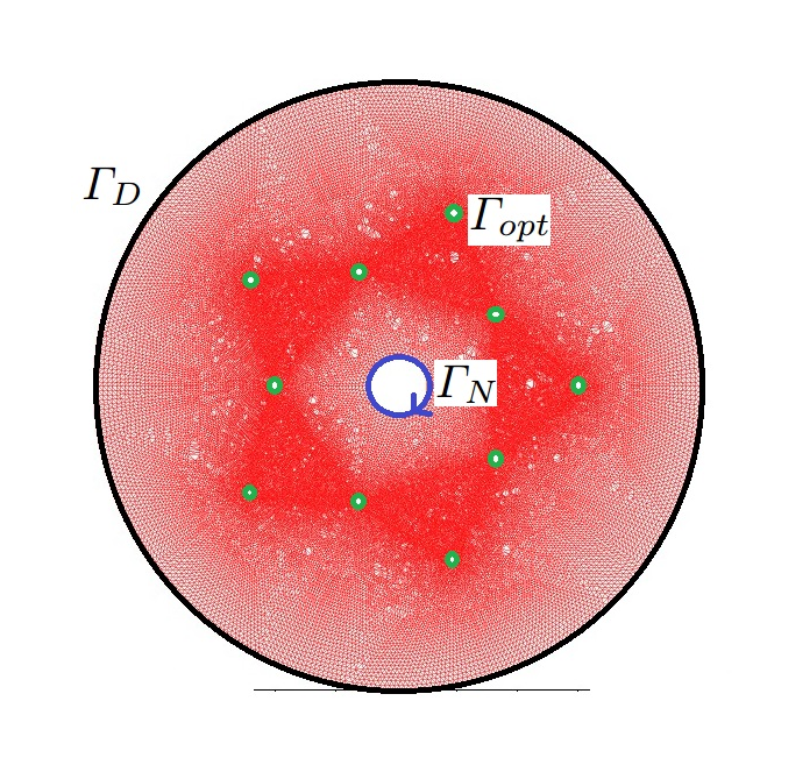
\includegraphics[width=0.6\textwidth]{w0.png}
\caption{Mô phỏng lực tác dụng lên vành bánh xe.}
\label{fig:w0}
\end{figure}\\
Trong đó:
\begin{itemize}
\item Biên $\Gamma_N$ chịu tác dụng của lực quay của trục xe.
\item Giả sử trong thời gian ngắn, vành bánh xe được giữ cố định. Do đó ta đặt biên $\Gamma_D$ ở vành bánh xe.
\item $\Gamma_{opt}$ là phần biên ta cần tối ưu.
\end{itemize}
Sau khi chạy thuật toán ta thu được hình dạng của vành bánh xe như sau:
\begin{figure}[http]
\centering
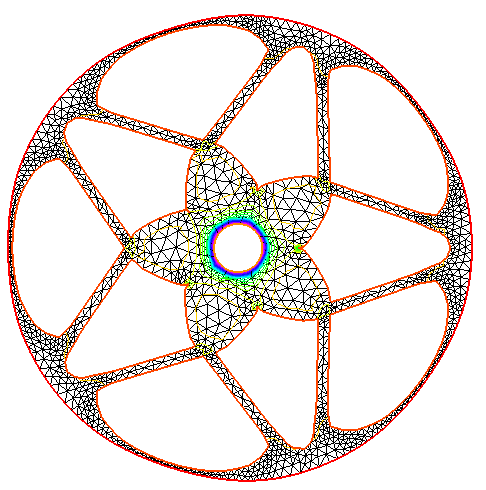
\includegraphics[width=0.5\textwidth]{w4.png}
\caption{Hình dạng vành bánh xe tối ưu.}
\label{fig:w0}
\end{figure}\\
Ta có thể thấy hình dạng tối ưu của vành bánh xe có sự tương đồng với vành bánh xe trên thực tế (hình \ref{fig:vanhtt}). Nhưng khi ta tăng thể tích ràng buộc lên thì ta lại được một kết quả tối ưu khác có phần hơi khác so với thực tế (hình \ref{fig:vanhtu}).
\begin{figure}[http]
\centering
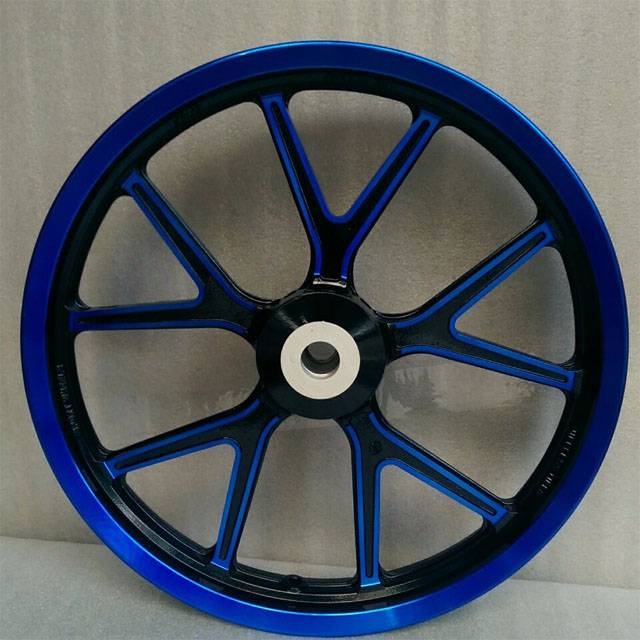
\includegraphics[width=0.5\textwidth]{w4.jpg}
\caption{Vành bánh xe.}\label{fig:vanhtt}
\label{fig:w0}
\end{figure}\\
\begin{figure}[http]
\centering
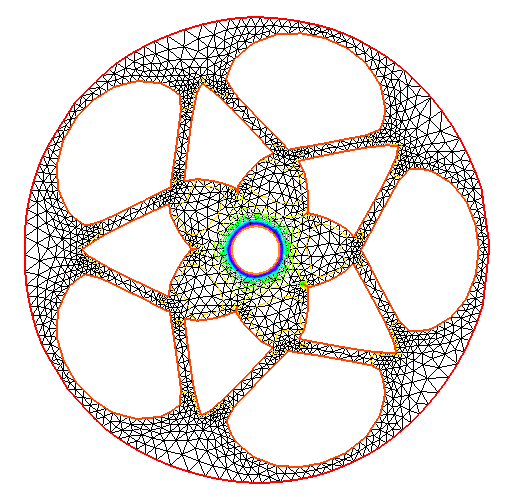
\includegraphics[width=0.5\textwidth]{w3.png}
\caption{Kết quả vành bánh xe tối ưu sau khi tăng thể tích $V_0$.}\label{fig:vanhtu}
\label{fig:w0}
\end{figure}\\

Tương tự như trên, ta thay đổi hình dạng ban đầu của vành bánh xe (hình \ref{fig:vanh3l}). Ta sẽ được một dạng tối ưu khác của vành bánh xe (hình \ref{fig:vanh3ltu}) và thực tế của chúng (hình \ref{fig:vanh3ltt}).
\begin{figure}[http]
\centering
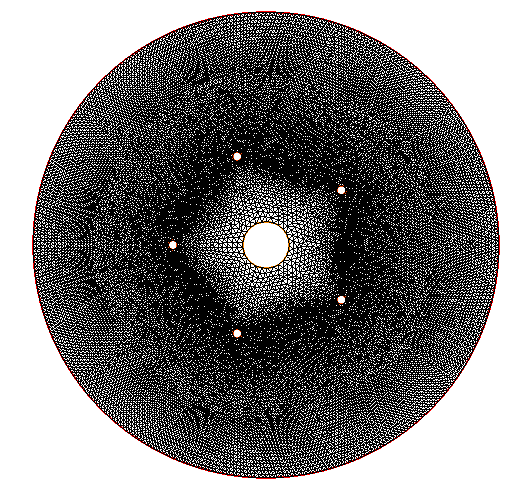
\includegraphics[width=0.5\textwidth]{w1.png}
\caption{Hình dạng ban đầu của vành bánh xe.}\label{fig:vanh3l}
\label{fig:w0}
\end{figure}\\
\begin{figure}[http]
\centering
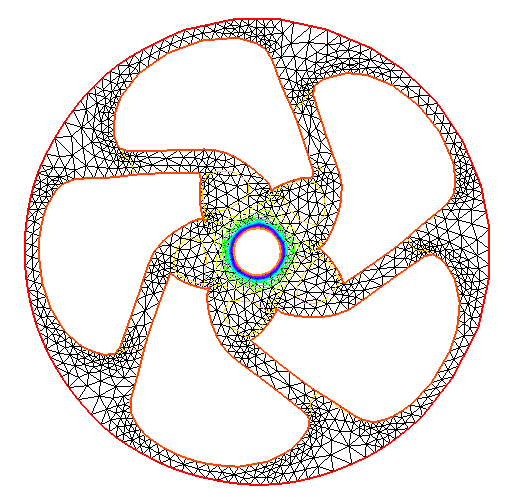
\includegraphics[width=0.5\textwidth]{w2.png}
\caption{Kết quả vành bánh xe tối ưu.}\label{fig:vanh3ltu}
\label{fig:w0}
\end{figure}\\
\begin{figure}[http]
\centering
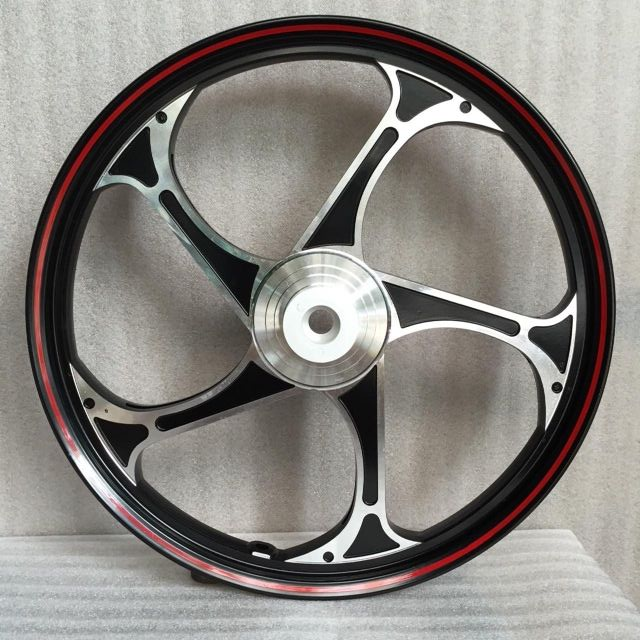
\includegraphics[width=0.5\textwidth]{w5.jpg}
\caption{Vành bánh xe trên thực tế.}\label{fig:vanh3ltt}
\label{fig:w0}
\end{figure}\\
%-----------------------------------------------------------
\section{Kết luận}
Trong chương này, ta đã giới thiệu bái toán tối ưu dạng cho phương trình đàn hồi. Cụ thể như sau:
\begin{itemize}
\item Giới thiệu bài toán tối ưu dạng cho phương trình đàn hồi.
\item Giới thiệu thuật toán để giải bài toán tối ưu dạng.
\item Trình bày các ví dụ mô phỏng cho bài toán tối ưu dạng.
\end{itemize}


\chapter*{\centering Kết luận chung} % Main chapter title 
\addstarredchapter{Kết luận chung}
Luận văn này trình bày một lược đồ giải số cho bài toán biến dạng đàn hồi và giới thiệu bài toán tối ưu dạng cho phương trình đàn hồi. Cụ thể, luận văn đã giải quyết những vấn đề sau:
\begin{itemize}
\item Xây dựng lược đồ mô phỏng số cho hệ phương trình đàn hồi dựa trên phương pháp phần tử hữu hạn. Có thể dễ dàng mở rộng cho các mô hình cơ học khác như phương trình đàn hồi phi tuyến, tải trọng phụ thuộc hình dạng của vật.
\item Ứng dụng của phương trình đàn hồi trong công nghiệp vật liệu.
\item Giới thiệu thuật toán giải số cho bài toán tối ưu dạng cho phương trình đàn hồi.
\item Mô phỏng các thí nghiệm giải số minh họa.
\end{itemize}

\chapter*{\centering Các hướng nghiên cứu tiếp theo}
\addstarredchapter{Các hướng nghiên cứu tiếp theo}
Tác giả đề xuất các hướng nghiên cứu liên quan có thể tiếp tục phát triển từ nội dung của luận văn này:
\begin{itemize}
\item Mô phỏng các thí nghiệm giải số cho hệ phương trình đàn hồi tuyến tính hoặc phi tuyến cũng như cho bài toán tối ưu dạng trong không gian ba chiều.
\item Nghiên cứu thêm về các lược đồ để giải quyết các bài toán ứng dụng tối ưu dạng trong nhiều mô hình vật lý khác nhau, chẳng hạn như cấu trúc truyền nhiệt \cite{YWM13}, dòng đối lưu tự nhiên \cite{AAA+14}, dòng chảy Navier-Stokes \cite{DMZ08b}, các bài toán khác liên quan đến đàn hồi \citep{TG85}, \citep{Sad05}.
\end{itemize}

Dựa trên cách tiếp cận của thuật toán đề xuất, trong quá trình thực hiện luận văn này, tác giả đã nghiên cứu xây dựng lược đồ giải số cho bài toán tối ưu dạng trong cấu trúc đàn hồi tuyến tính và đã đạt được những kết quả nhất định. Tuy nhiên, do hạn chế về thời gian thực hiện nên nghiên cứu này vẫn đang trong quá trình tiếp tục hoàn thiện.

\chapter*{\centering Danh mục các công trình liên quan đến luận văn đã công bố}
\addstarredchapter{Danh mục các công trình liên quan đến luận văn đã công bố}
\begin{itemize}
\item[1.] T.T.Mai Ta, L.Hoang Nguyen, T.Hung Nguyen and X.Ly Le. “Simulation of linear elastic equation and application in mechanics of materials”. \textit{Applied Journal of Mathematical Applications}. Vol. XVI, No2, 2018, pp. 37-50.
\item[2.] “Linear elastic deformations and its application in shape design“, (preprint).
\end{itemize}

\printbibliography
\addstarredchapter{Tài liệu tham khảo}


%----------------------------------------------------------------------------------------
\end{document}  
